\documentclass[12pt,a4paper,oneside]{article}

\usepackage{fontspec}
\setmainfont{Times New Roman}
\usepackage[vietnamese]{babel}
\usepackage[a4paper,left=2.7cm,right=2.2cm,top=2.1cm,bottom=2.0cm,headheight=16pt]{geometry}
\usepackage{graphicx}
\usepackage{booktabs}
\usepackage{array}
\usepackage{float}
\usepackage{caption}
\usepackage{enumitem}
\usepackage{fancyhdr}
\usepackage{xcolor}
\usepackage{tikz}
\usetikzlibrary{calc,positioning,arrows.meta}
\usepackage{lastpage}
\usepackage{hyperref}
\usepackage{tabularx}

\definecolor{hcmutblue}{HTML}{003DA5}
\hypersetup{
  colorlinks=true,
  linkcolor=black,
  urlcolor=hcmutblue,
  pdftitle={Báo cáo đồ án tốt nghiệp học kỳ 261},
  pdfauthor={Nguyễn Vũ Quang Minh}
}
\renewcommand{\contentsname}{Mục lục}
\setlength{\parskip}{0.35em}
\setlength{\parindent}{1em}
\setlength{\tabcolsep}{4pt}
\emergencystretch=2em
\renewcommand{\arraystretch}{1.2}

\setlist[itemize]{leftmargin=1.5em,itemsep=0.15em,topsep=0.2em}
\setlist[enumerate]{leftmargin=1.7em,itemsep=0.15em,topsep=0.2em}
\captionsetup{font=small,labelfont=bf,skip=3pt}
\setlength{\textfloatsep}{8pt plus 2pt minus 2pt}
\setlength{\intextsep}{7pt plus 2pt minus 2pt}
\pagestyle{fancy}
\fancyhf{}
\fancyhead[L]{Báo cáo tiến độ đồ án tốt nghiệp}
\fancyhead[R]{HK 261 | 2026--2027}
\fancyfoot[L]{\small HK261-DATN-021}
\fancyfoot[R]{\small Trang \thepage/\pageref{LastPage}}
\renewcommand{\headrulewidth}{0.35pt}
\renewcommand{\footrulewidth}{0.35pt}

\begin{document}

% Bìa tiếng Việt, giữ thứ tự khối và viền đôi theo mẫu báo cáo HK252.
\begin{titlepage}
\thispagestyle{empty}
\begin{tikzpicture}[remember picture,overlay]
  \draw[line width=3.2pt]
    ($(current page.north west)+(0.40in,-0.42in)$)
    rectangle
    ($(current page.south east)+(-0.40in,0.42in)$);
  \draw[line width=1.1pt]
    ($(current page.north west)+(0.46in,-0.48in)$)
    rectangle
    ($(current page.south east)+(-0.46in,0.48in)$);
\end{tikzpicture}

\centering
\vspace*{0.72cm}
{\large\bfseries ĐẠI HỌC QUỐC GIA THÀNH PHỐ HỒ CHÍ MINH\par}
\vspace{0.12cm}
{\large\bfseries TRƯỜNG ĐẠI HỌC BÁCH KHOA\par}
\vspace{0.12cm}
{\large\bfseries KHOA KHOA HỌC VÀ KỸ THUẬT MÁY TÍNH\par}
\vspace{0.28cm}
{\normalsize HK261-DATN-021\par}
\vspace{0.30cm}

\includegraphics[width=2.55cm]{assets/hcmut-logo.png}\par
\vspace{0.22cm}
{\Large\bfseries BÁO CÁO TIẾN ĐỘ GIỮA KỲ \par}
\vspace{0.08cm}
{\LARGE\bfseries ĐỒ ÁN TỐT NGHIỆP\par}
\vspace{0.08cm}
{\large\bfseries HỌC KỲ 261 -- NĂM HỌC 2026--2027\par}
\vspace{0.30cm}
\rule{0.83\textwidth}{0.45pt}\par
\vspace{0.24cm}
{\Large\bfseries\color{hcmutblue}
Transformer Đa phương thức cho Dự báo Nhu cầu Bán lẻ\\
trong Điều kiện Một số Phương thức Dữ liệu bị Thiếu\par}
\vspace{0.24cm}
\rule{0.83\textwidth}{0.45pt}\par
\vspace{0.40cm}
{\large\bfseries NGÀNH: KHOA HỌC MÁY TÍNH\par}
\vspace{0.42cm}
\begin{tabular}{>{\centering\arraybackslash}p{0.82\textwidth}}
  \textbf{GIẢNG VIÊN HƯỚNG DẪN}\\[0.10cm]
  TS. TRƯƠNG VĨNH LÂN (004343)\\[0.40cm]
  \textbf{SINH VIÊN THỰC HIỆN}\\[0.10cm]
  NGUYỄN VŨ QUANG MINH (2212071)
\end{tabular}

\vfill
{\large TP. HỒ CHÍ MINH, THÁNG 10 NĂM 2026\par}
\vspace{0.65cm}
\end{titlepage}

\pagenumbering{roman}
\clearpage
\tableofcontents
\clearpage
\pagenumbering{arabic}

\section{Giới thiệu đề tài}
\subsection{Bối cảnh và lý do chọn đề tài}
Trong bán lẻ thời trang, lượng bán của một mặt hàng thay đổi theo mùa, xu hướng, giá bán và đặc điểm của sản phẩm. Khi lịch sử giao dịch ngắn hoặc thưa, chỉ dựa vào các tuần đã bán có thể chưa đủ để mô tả một mặt hàng. Mặt khác, doanh nghiệp thường có thêm tên, nhóm, mô tả và hình ảnh sản phẩm. Đây là cơ sở để khảo sát liệu thông tin đa phương thức có giúp cải thiện dự báo hay không, và mức độ ảnh hưởng khi một nguồn đầu vào không có sẵn.

Đồ án chọn bộ dữ liệu H\&M vì dữ liệu giao dịch có thể liên kết với metadata và ảnh bằng mã sản phẩm. Cấu trúc này cho phép xây dựng bài toán dự báo theo mặt hàng-tuần, lập các baseline chỉ dùng chuỗi bán hàng và mở rộng sang mô hình kết hợp ảnh, văn bản. Quy mô dữ liệu cũng đủ lớn để khảo sát tình trạng giao dịch thưa và sự khác biệt giữa nhóm sản phẩm.

Về mặt ứng dụng, dự báo ở cấp sản phẩm có thể hỗ trợ lập kế hoạch phân bổ hàng và nhận diện mặt hàng có biến động bán. Tuy nhiên, giao dịch quan sát không đồng nhất với nhu cầu thực: khi sản phẩm hết hàng, lượng bán ghi nhận có thể thấp hơn nhu cầu. Báo cáo vì thế dùng cách gọi \emph{lượng bán quan sát} cho biến đích và tránh suy rộng kết quả thành dự báo nhu cầu không bị giới hạn bởi tồn kho.

Đề tài còn có ý nghĩa phương pháp luận. Các sản phẩm mới hoặc ít giao dịch thường có chuỗi lịch sử ngắn, trong khi metadata và ảnh có thể cung cấp tín hiệu bổ sung về loại, nhóm và đặc điểm trực quan. Mặt khác, ảnh có thể không tồn tại, mô tả có thể trống, hoặc dữ liệu của một modality có thể không được truyền đến hệ thống dự báo. Vì vậy ngoài việc so sánh sai số khi có đủ đầu vào, cần đánh giá có kiểm soát khi từng nguồn bị thiếu. Kết quả Stage 3 hiện mới cung cấp baseline và phép thử độ nhạy; cơ chế học để tự thích nghi với missing modality sẽ được xây dựng ở giai đoạn tiếp theo.

\subsection{Mục tiêu, câu hỏi và phạm vi}
Mục tiêu ở giai đoạn hiện tại là hoàn thiện quy trình dữ liệu có thể tái lập, đo baseline theo cùng một phép chia thời gian, sau đó dùng kết quả làm mốc cho kiến trúc đa phương thức và thử nghiệm thiếu modality. Những câu hỏi nghiên cứu định hướng gồm:
\begin{enumerate}
  \item Các mô hình học chuỗi thời gian có cải thiện sai số so với dự báo ngây thơ trên cùng tập kiểm tra không?
  \item Khi giữ nguyên trọng số đã huấn luyện, việc bỏ ảnh, văn bản hoặc cả hai làm thay đổi sai số bao nhiêu?
  \item Một kiến trúc đa phương thức được huấn luyện có chủ đích với modality dropout có bền vững hơn baseline hiện tại không?
\end{enumerate}
Câu hỏi thứ ba chưa được trả lời trong kết quả hiện tại. Phạm vi báo cáo là tiến độ và bằng chứng đã có đến hết giai đoạn baseline; không xem các ý tưởng kiến trúc ở giai đoạn sau là kết quả đã thực nghiệm.

Ba câu hỏi được gắn với các bằng chứng khác nhau. Câu hỏi thứ nhất được trả lời bằng bảng baseline trên cùng split thời gian. Câu hỏi thứ hai dùng \texttt{same\_checkpoint}: giữ nguyên trọng số của Multimodal MLP rồi che một hay nhiều đầu vào khi đánh giá. Câu hỏi thứ ba cần một mô hình mới được huấn luyện với chiến lược che modality, cùng đối chứng có kiểm soát; kết quả này hiện chưa có. Cách tách câu hỏi ngăn việc diễn giải một phép thay vector bằng 0 sau huấn luyện như bằng chứng cho khả năng tự bù thông tin.

\begin{table}[!htbp]
\centering
\caption{Phạm vi bài toán tại thời điểm báo cáo.}
\label{tab:scope}
\begin{tabular}{p{0.25\textwidth}p{0.65\textwidth}}
\toprule
Thành phần & Định nghĩa / phạm vi hiện tại \\
\midrule
Đơn vị quan sát & Một sản phẩm trong một tuần ISO. \\
Biến mục tiêu & Số dòng giao dịch quan sát được của sản phẩm trong tuần. \\
Đầu vào đã có & 12 tuần lịch sử; embedding ảnh và văn bản cho baseline đa phương thức. \\
Chân trời dự báo & Hai tuần tiếp theo, $H=2$. \\
Ngoài phạm vi kết luận & Nhu cầu bị mất do hết hàng, tác động nhân quả của giá/khuyến mãi và dự báo cho mặt hàng hoàn toàn mới. \\
\bottomrule
\end{tabular}
\end{table}

\subsection{Định nghĩa bài toán dự báo}
Gọi $i$ là mã sản phẩm và $w$ là tuần ISO. Biến mục tiêu được xây dựng từ các dòng giao dịch quan sát:
\begin{equation}
 y_{i,w}=\sum_{r\in\mathcal{R}}\mathbf{1}\bigl[\mathrm{article}(r)=i\;\land\;\mathrm{week}(r)=w\bigr].
 \label{eq:weekly-sales}
\end{equation}
Với mỗi cửa sổ dự báo tại thời điểm gốc $t$, mô hình nhận chuỗi
$\mathbf{x}_{i,t}=(y_{i,t-L+1},\ldots,y_{i,t})$ và dự báo
$\hat{\mathbf{y}}_{i,t}=(\hat y_{i,t+1},\ldots,\hat y_{i,t+H})$, trong đó $L=12$ và $H=2$ ở thực nghiệm hiện tại. Cặp $(i,t)$ là một mẫu; do đó 88.000 cửa sổ test không có nghĩa là 88.000 mặt hàng riêng biệt.

Trong panel cân bằng, mọi sản phẩm được biểu diễn ở mọi tuần trong lưới 104 tuần. Nếu không có dòng giao dịch cho cặp $(i,w)$ thì $y_{i,w}=0$. Đây là quy ước phục vụ mô hình hóa chuỗi trên lưới đều, không phải nhãn xác nhận rằng nhu cầu tiềm ẩn bằng 0. Cách diễn giải này đặc biệt quan trọng khi đánh giá các mô hình trên mặt hàng thưa hoặc có khả năng hết hàng.

\section{Nguồn dữ liệu và quy trình xây dựng}
\subsection{Nguồn và căn cứ lựa chọn}
Dữ liệu gốc là bộ \href{https://www.kaggle.com/competitions/h-and-m-personalized-fashion-recommendations}{H\&M Personalized Fashion Recommendations trên Kaggle}. Notebook được sử dụng trong quá trình triển khai là \href{https://www.kaggle.com/code/alexnguyen147/datn-notebook}{notebook DATN của sinh viên}. Bộ dữ liệu có ba thành phần thiết yếu: giao dịch theo ngày và mã sản phẩm, bảng thuộc tính sản phẩm, cùng ảnh sản phẩm theo mã. Các thành phần có thể được ghép bằng \texttt{article\_id}, giảm nhu cầu tạo nhãn thủ công.

Dữ liệu chứa 31.788.324 dòng giao dịch từ ngày 20/09/2018 đến 22/09/2020. Khoảng ngày quan sát trải qua 106 tuần lịch; để tránh tuần đầu/cuối chỉ có một phần ngày, pipeline giữ lại 104 tuần trọn vẹn. Mốc cuối cùng trong lưới phân tích là tuần 2020-W38. Việc loại tuần biên được áp dụng nhất quán trước khi chia train, validation và test.

\subsection{Từ giao dịch thô đến ma trận nhu cầu tuần}
Mỗi dòng trong bảng giao dịch được xem là một giao dịch quan sát. Pipeline đọc dữ liệu theo từng phần, chuyển ngày sang tuần ISO, sau đó đếm số dòng theo cặp sản phẩm-tuần. Tiếp theo, hệ thống tạo tích Descartes giữa danh sách sản phẩm được chọn và 104 tuần; những cặp không có giao dịch được điền 0. Do đó, một số 0 có ý nghĩa ``không ghi nhận giao dịch'', không mặc nhiên có nghĩa ``không có nhu cầu''.

Tuần ISO được dùng để thống nhất ranh giới lịch giữa các năm. Mỗi ngày giao dịch được ánh xạ sang cặp năm-tuần ISO trước khi tổng hợp; sau bước này, phép nhóm theo \texttt{article\_id} và tuần chỉ đếm số bản ghi trong nhóm. Hai tuần biên không đủ bảy ngày bị loại để mỗi cột thời gian trong panel đại diện cho một khoảng tuần đầy đủ. Chính sách này tránh so sánh một tuần quan sát một phần với tuần đầy đủ, dù đồng thời làm phạm vi panel ngắn hơn khoảng ngày gốc.

Quy trình có thể được nhìn như bốn phép biến đổi liên tiếp: chuẩn hóa khóa và lịch; tổng hợp đếm theo sản phẩm-tuần; hoàn thiện lưới bằng zero-fill; rồi tạo cửa sổ lịch sử-mục tiêu theo ranh giới split. Việc tách các bước giúp kiểm tra lỗi theo từng tầng: số giao dịch phải bảo toàn sau tổng hợp, mỗi khóa sản phẩm-tuần chỉ có một giá trị, panel phải đủ 104 tuần cho mỗi sản phẩm và không có cửa sổ nào lấy target bắc qua ranh giới tập.

\begin{figure}[!htbp]
\centering
\begin{tikzpicture}[
  box/.style={draw=hcmutblue,rounded corners=2pt,fill=blue!4,align=center,
              text width=3.05cm,minimum height=1.25cm,font=\small,inner sep=5pt},
  arrow/.style={-{Stealth[length=2.2mm]},thick,hcmutblue}]
  \node[box] (raw) {Giao dịch thô\\ngày, mã sản phẩm};
  \node[box,right=0.55cm of raw] (weekly) {Tổng hợp theo\\tuần ISO};
  \node[box,right=0.55cm of weekly] (panel) {Panel cân bằng\\8.000 x 104 tuần};
  \node[box,right=0.55cm of panel] (window) {Cửa sổ\\$L=12$, $H=2$};
  \draw[arrow] (raw) -- (weekly);
  \draw[arrow] (weekly) -- (panel);
  \draw[arrow] (panel) -- (window);
  \node[below=0.28cm of weekly,align=center,text width=3.4cm,font=\footnotesize]
       {Đếm bản ghi theo\\(sản phẩm, tuần)};
  \node[below=0.28cm of panel,align=center,text width=3.4cm,font=\footnotesize]
       {Bổ sung tuần không bán\\và lịch tuần};
  \node[below=0.28cm of window,align=center,text width=3.6cm,font=\footnotesize]
       {Chỉ giữ cửa sổ có\\target trong cùng split};
\end{tikzpicture}
\caption{Luồng chuyển từ giao dịch sang mẫu học; zero-fill biểu diễn không ghi nhận bán trong panel.}
\label{fig:data-pipeline}
\end{figure}

Ở bước cuối, mỗi cặp sản phẩm-vị trí dự báo tạo ra một mẫu độc lập về mặt cấu trúc. Với 8.000 sản phẩm và 11 origin hợp lệ trong validation hoặc test, số mẫu mỗi tập là $8.000\times 11=88.000$. Vì hai giá trị đích được phát ra cho mỗi mẫu, mỗi tập kiểm tra có 176.000 cặp giá trị thật-dự báo khi tính metric gộp. Đây là số điểm dự báo, không phải kích thước tập sản phẩm mới.

\begin{figure}[!htbp]
\centering
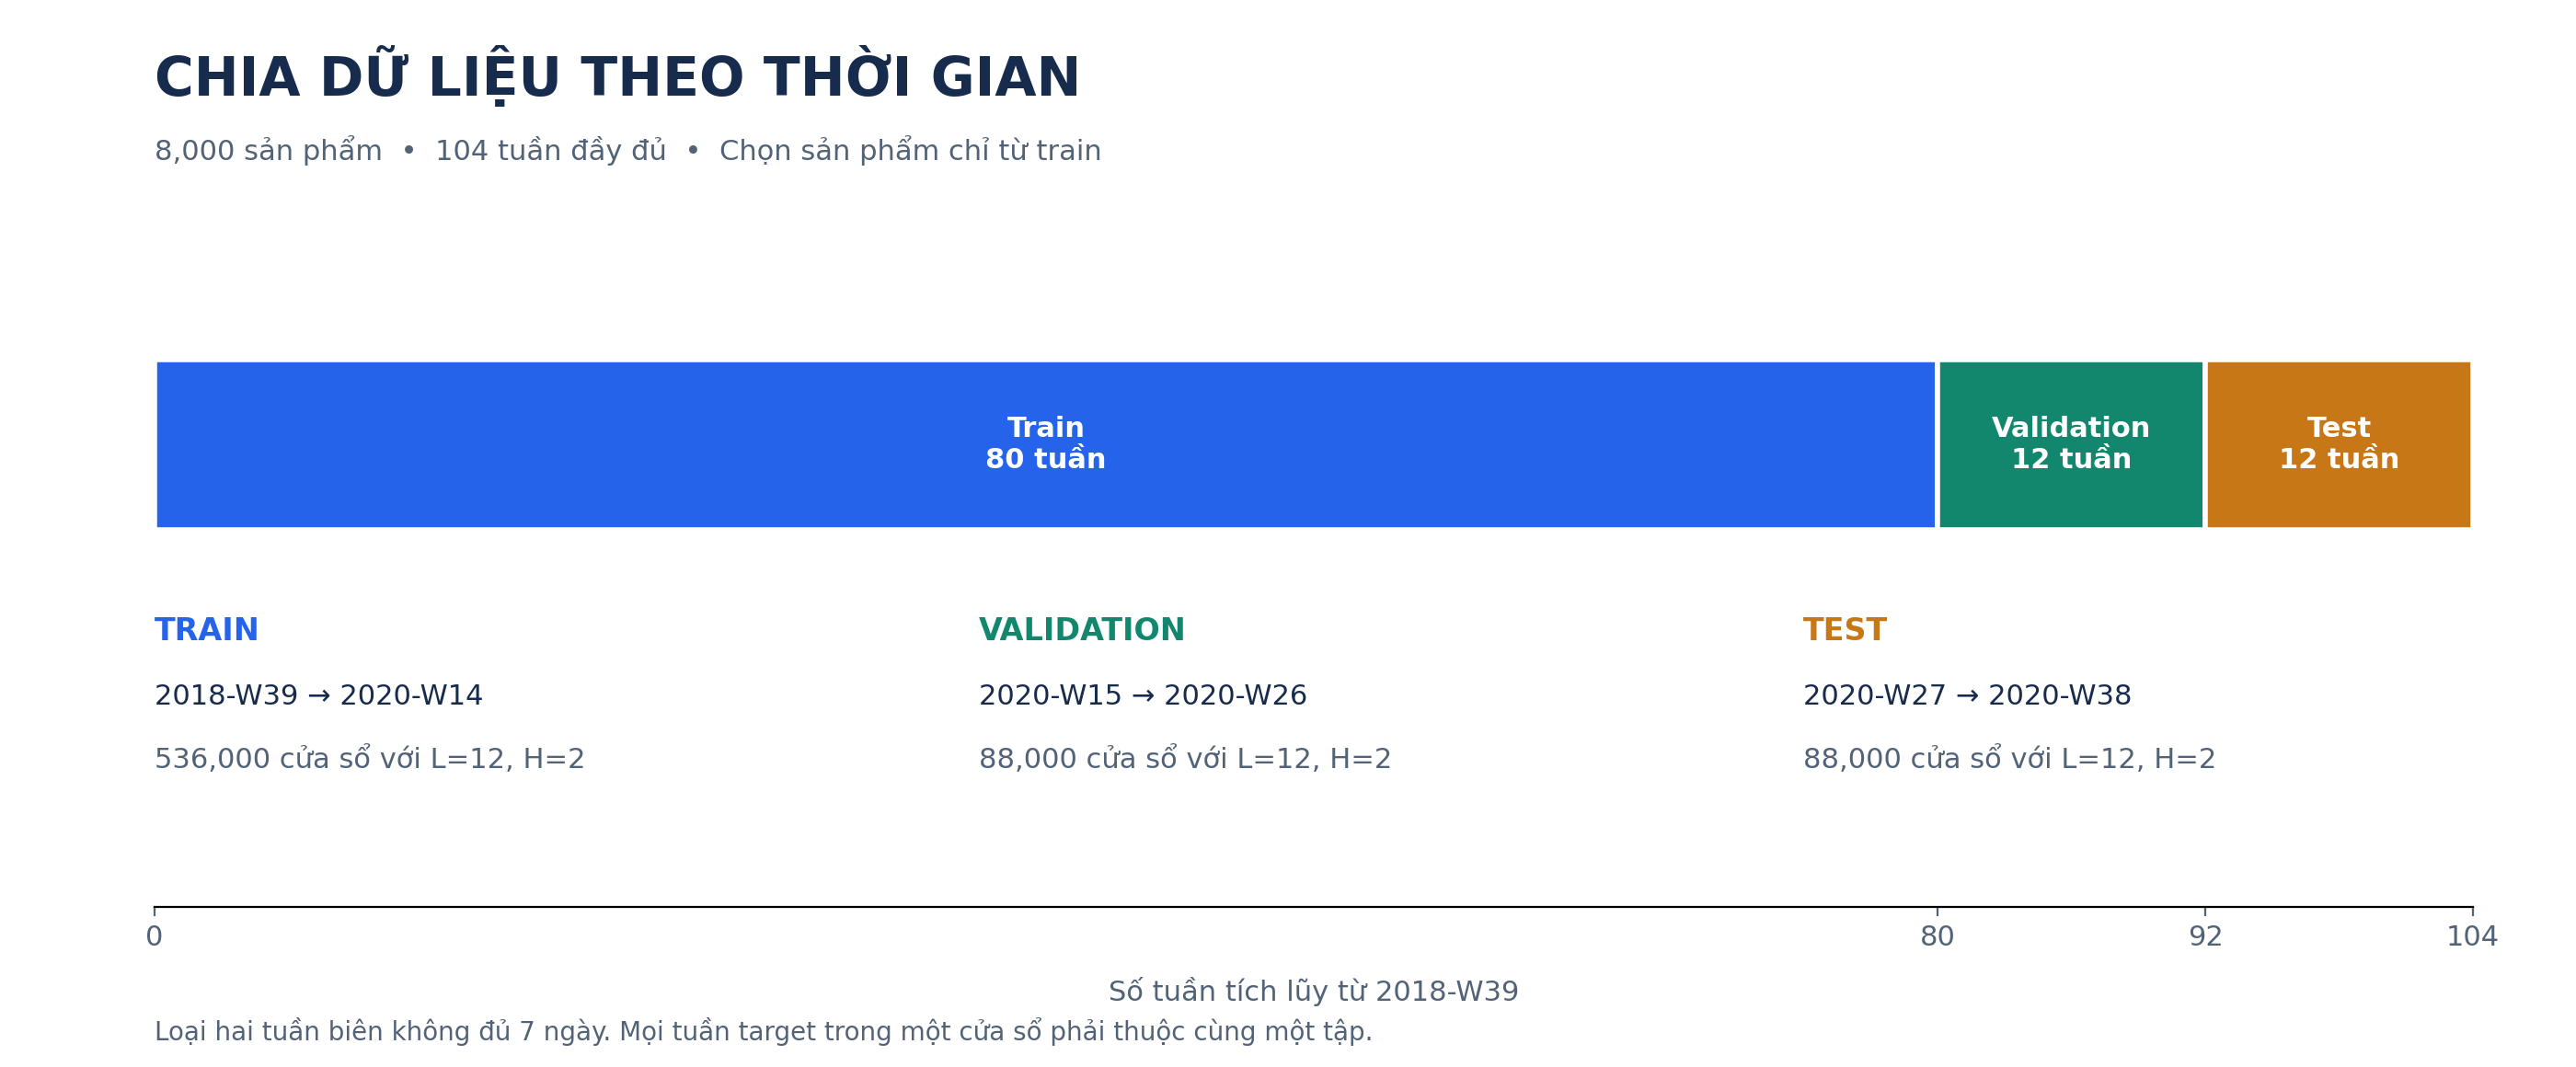
\includegraphics[width=0.84\textwidth]{../../docs/figures/time_split_v2.png}
\caption{Trình tự chia theo thời gian và số cửa sổ dự báo ở mỗi tập.}
\label{fig:split}
\end{figure}

\begin{figure}[!htbp]
\centering
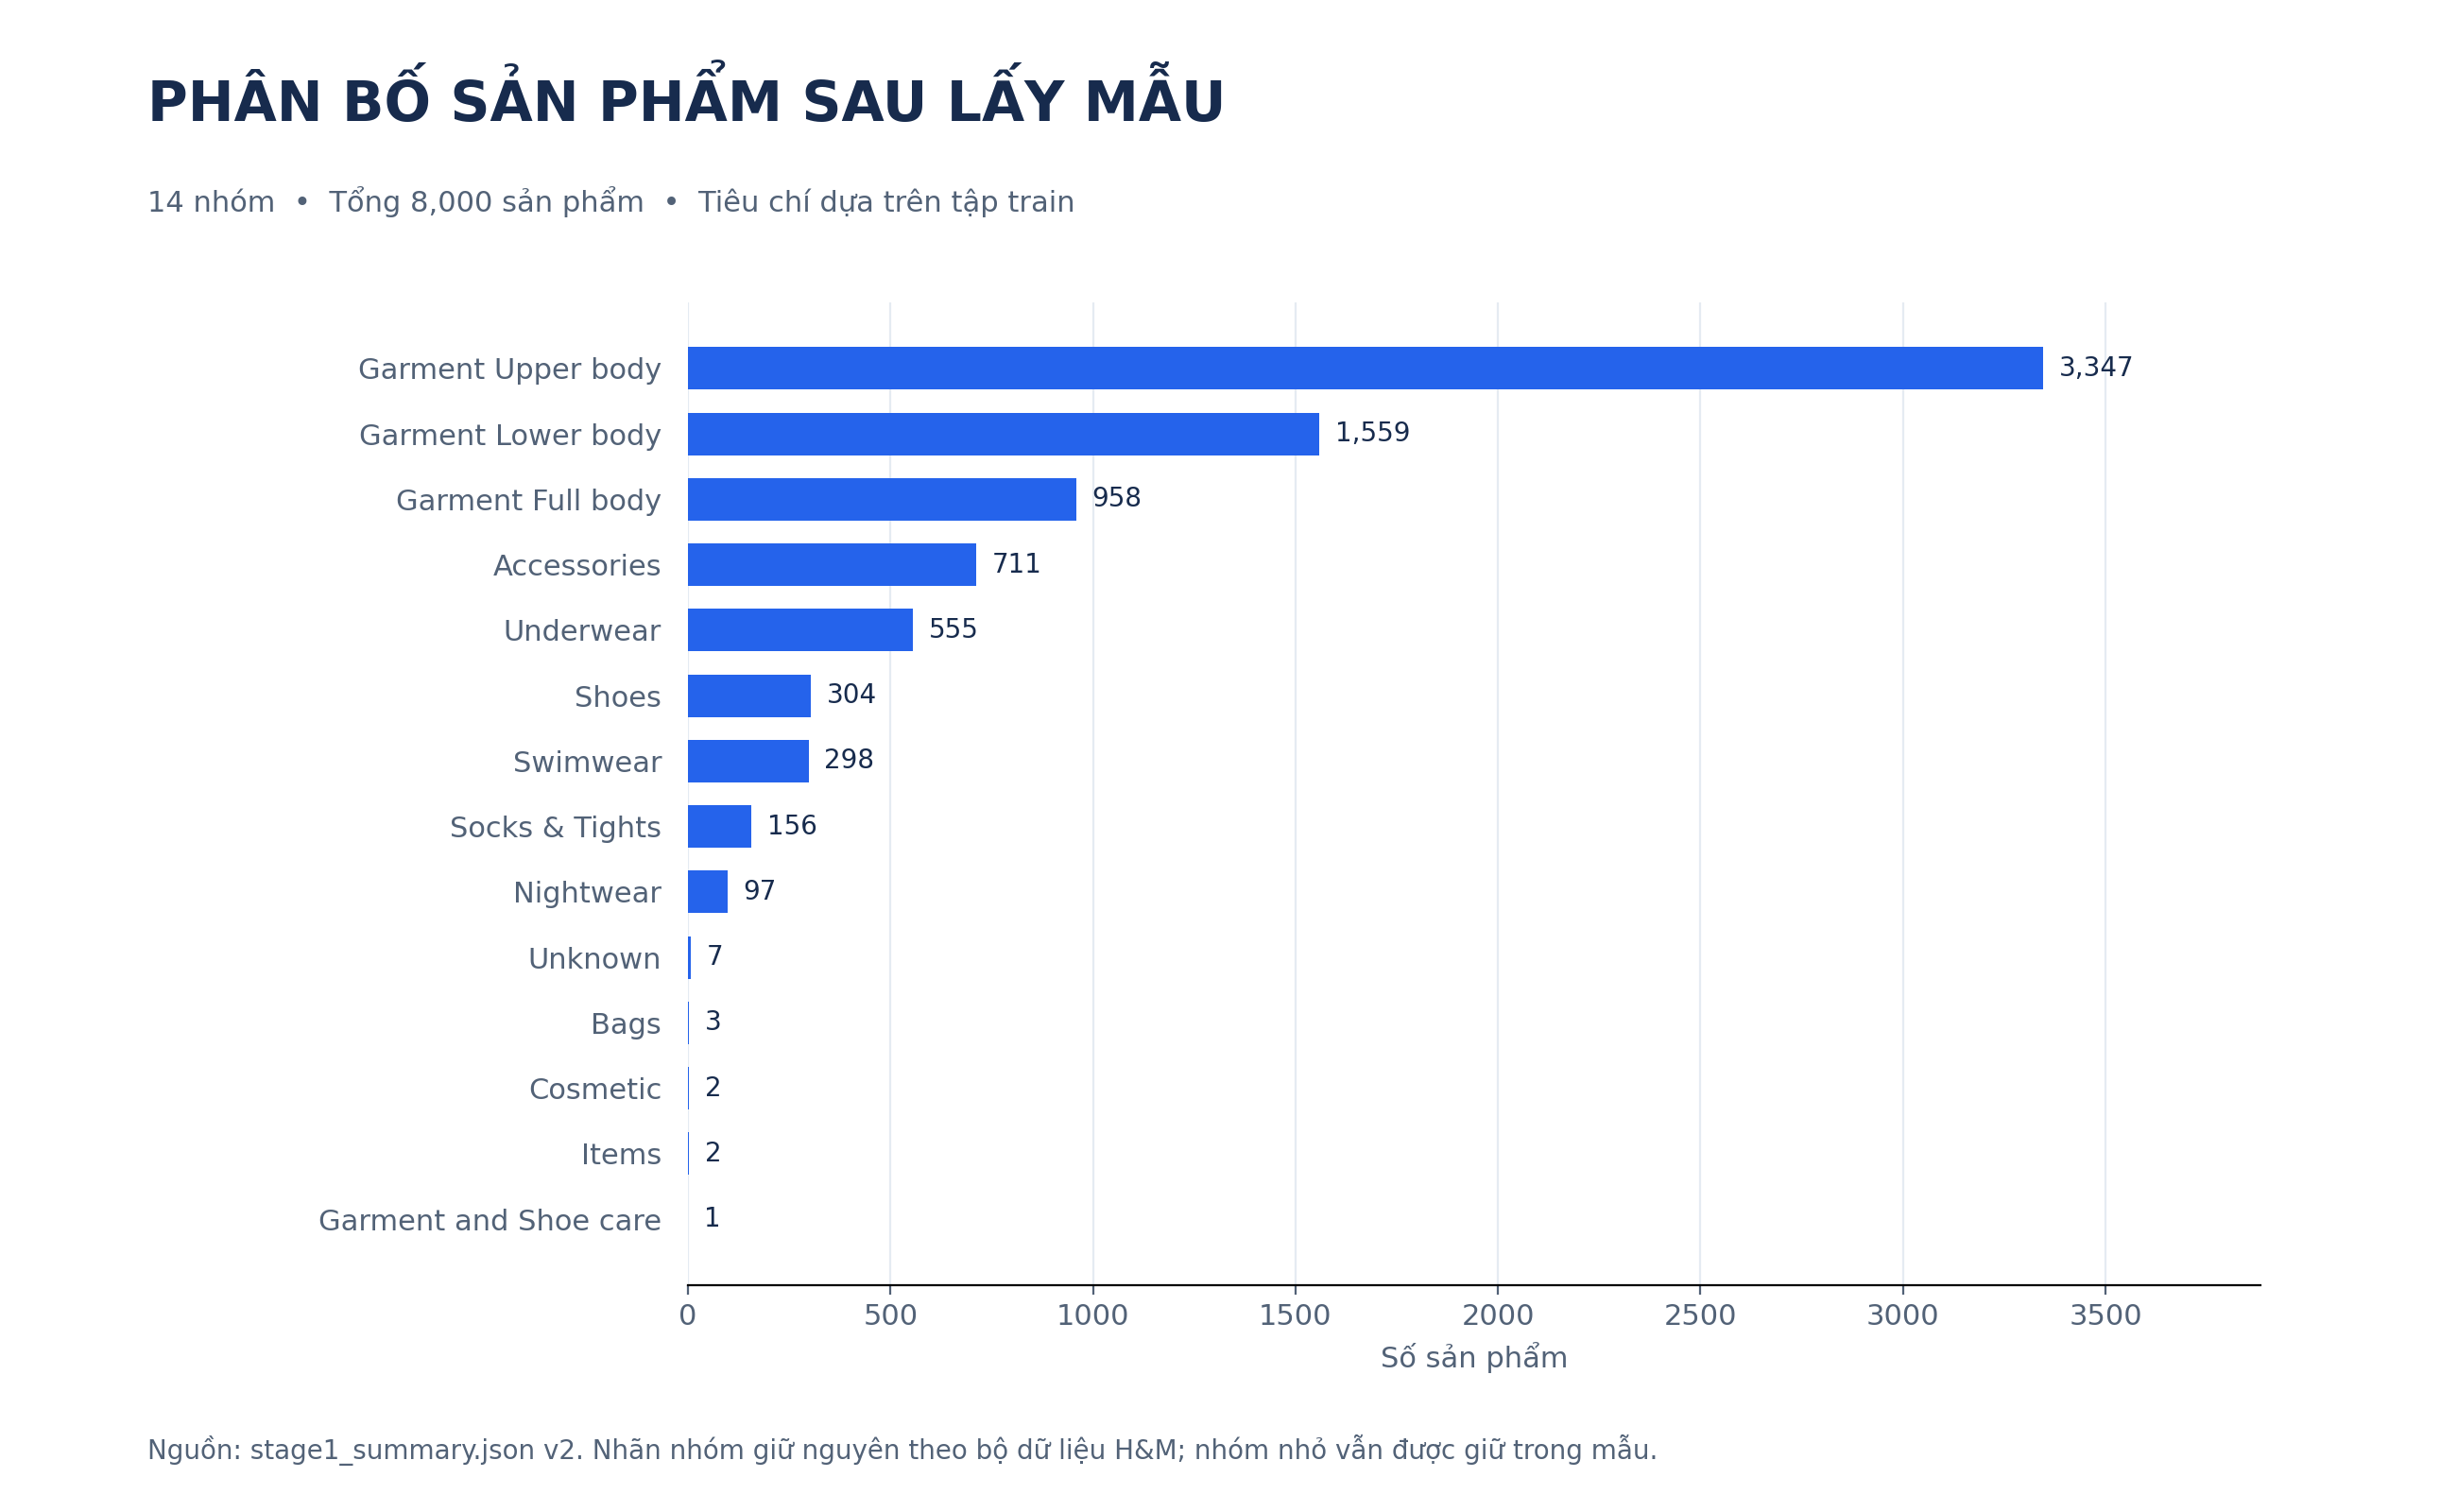
\includegraphics[width=0.88\textwidth]{../../docs/figures/product_groups_v2.png}
\caption{Phân bố 8.000 sản phẩm mẫu theo 14 nhóm sau lấy mẫu phân tầng; nhóm nhỏ vẫn được giữ trong mẫu.}
\label{fig:product-groups}
\end{figure}

Hình \ref{fig:product-groups} cho thấy phân tầng không làm cho các nhóm có cùng kích thước. Nhóm ``Garment Upper body'' chiếm 3.347 sản phẩm, trong khi một số nhóm chỉ có một vài mã. Điều này phản ánh phân bố sản phẩm trong tập ứng viên và nhắc rằng metric gộp chủ yếu chịu ảnh hưởng từ nhóm lớn. Khi hoàn tất nghiên cứu, nên báo cáo thêm sai số theo nhóm, đồng thời ghi rõ các nhóm có số mẫu quá nhỏ để tránh kết luận mạnh từ vài mặt hàng.

\begin{table}[!htbp]
\centering
\small
\caption{Một số quy mô nhóm trong mẫu sản phẩm được chọn.}
\label{tab:group-counts}
\begin{tabular}{lr}
\toprule
Nhóm sản phẩm & Số mã trong 8.000 sản phẩm \\
\midrule
Garment Upper body & 3.347 \\
Garment Lower body & 1.559 \\
Garment Full body & 958 \\
Accessories & 711 \\
Underwear & 555 \\
Shoes & 304 \\
Tám nhóm còn lại & 566 \\
\bottomrule
\end{tabular}
\end{table}

Nhóm ``Tám nhóm còn lại'' là tổng của Swimwear, Socks \& Tights, Nightwear, Unknown, Bags, Items, Cosmetic và Garment and Shoe care; đây không phải nhãn gốc mới. Nhóm lớn nhất chiếm hơn 40\% số mã được chọn, trong khi nhiều nhóm nhỏ có dưới mười mã. Bảng dùng để nhấn mạnh mức lệch phân bố, không thay thế bảng đầy đủ 14 nhóm trong dữ liệu nguồn.

\subsection{Chọn sản phẩm và chia tập}
Tập ứng viên gồm 33.514 sản phẩm có hoạt động trong dữ liệu. Để tránh sử dụng thông tin tương lai khi chọn mẫu, số tuần hoạt động và tổng giao dịch chỉ được tính trong giai đoạn train. Sản phẩm phải có ít nhất 20 tuần hoạt động và 50 giao dịch; sau đó lấy mẫu 8.000 sản phẩm với seed 42 và phân tầng theo nhóm sản phẩm. Kết quả gồm 14 nhóm và 832.000 dòng sản phẩm-tuần. Trong lưới này, 60,1577\% giá trị mục tiêu bằng 0; con số này cho thấy dữ liệu thưa và cần thận trọng khi chỉ đọc metric tổng hợp.

Phép chia giữ thứ tự thời gian: 80 tuần train, 12 tuần validation và 12 tuần test. Tạo cửa sổ rolling-origin với 12 tuần lịch sử và 2 tuần dự báo cho mỗi sản phẩm cho ra lần lượt 536.000, 88.000 và 88.000 cửa sổ. Hai tuần mục tiêu của mỗi cửa sổ nằm trọn trong một split; vì vậy số mẫu là số cửa sổ sản phẩm-thời điểm, không phải số tuần lịch độc lập. Ở các origin sau trong tập đánh giá, các quan sát quá khứ đã xảy ra có thể được dùng làm lịch sử, phù hợp thiết lập dự báo rolling-origin.

\begin{table}[!htbp]
\centering
\caption{Tóm tắt dữ liệu và phép chia thực nghiệm.}
\label{tab:data}
\begin{tabular}{p{0.31\textwidth}p{0.59\textwidth}}
\toprule
Chỉ số & Giá trị đã ghi nhận \\
\midrule
Giao dịch gốc & 31.788.324; 20/09/2018--22/09/2020 \\
Tuần lịch & 106 tuần quan sát; giữ 104 tuần trọn vẹn \\
Mẫu sản phẩm & 8.000 từ 33.514 ứng viên; 14 nhóm \\
Lưới sau zero-fill & 832.000 dòng; tỷ lệ zero 60,1577\% \\
Train / validation / test & 80 / 12 / 12 tuần; 536.000 / 88.000 / 88.000 cửa sổ \\
Cửa sổ dự báo & $L=12$ tuần đầu vào; $H=2$ tuần dự báo \\
Thiếu mô tả ngắn & 38 sản phẩm trong mẫu thiếu \texttt{detail\_desc}. \\
\bottomrule
\end{tabular}
\end{table}

\subsection{Kiểm soát rò rỉ thông tin theo thời gian}
Trong dự báo chuỗi thời gian, chia ngẫu nhiên các cửa sổ có thể đặt các tuần gần nhau của cùng sản phẩm ở cả train và test. Cách chia như vậy dễ khiến đánh giá không phản ánh việc dự báo trong tương lai. Pipeline hiện tại giữ nguyên trật tự tuần, dùng giai đoạn đầu để huấn luyện, tiếp theo để chọn mô hình và giai đoạn cuối để đánh giá. Danh sách sản phẩm cũng được lọc dựa trên hoạt động và số giao dịch trong train thay vì sử dụng thống kê toàn bộ thời gian.

Thiết lập rolling-origin cho phép một quan sát đã trở thành quá khứ được dùng làm lịch sử ở một origin sau. Điều kiện cốt lõi là hai tuần target của từng cửa sổ luôn thuộc cùng split và không xuất hiện trong đầu vào của chính cửa sổ đó. Tập validation được dùng chọn checkpoint theo MAE; test chỉ được dùng sau khi đã hoàn thành lựa chọn mô hình. Hình \ref{fig:split} cùng các mốc ISO trong Bảng \ref{tab:data} mô tả quy ước này.

\section{Đặc trưng đa phương thức và kiểm định}
\subsection{Chuỗi bán hàng}
Chuỗi đầu vào gồm 12 số đếm tuần liên tiếp. Mục tiêu gồm lượng giao dịch của hai tuần tiếp theo. Dataset cũng chuẩn bị các thuộc tính lịch và cờ khả dụng embedding để những mô hình ở bước sau có thể dùng. Các baseline hiện tại không nhất thiết khai thác hết các trường này; báo cáo không diễn giải rằng chúng đã được mô hình sử dụng nếu cấu hình không đưa chúng vào.

Chuỗi bán hàng giữ nguyên đơn vị đếm trong dữ liệu sau tổng hợp. Đối với các mô hình học, target được biến đổi $\log(1+y)$ khi tối ưu để giảm chênh lệch thang đo giữa mặt hàng bán ít và mặt hàng bán nhiều; dự báo được đánh giá sau khi chuyển về đơn vị ban đầu. Vì phép biến đổi phi tuyến có thể làm thay đổi phân bố sai số, tất cả bảng metric trong báo cáo dùng dự báo sau nghịch biến đổi và target gốc, theo chính sách trong cấu hình run.

\subsection{Văn bản sản phẩm}
Văn bản được tạo từ tên sản phẩm, loại sản phẩm, nhóm sản phẩm và mô tả chi tiết. Mô tả thiếu được xử lý bằng chuỗi rỗng trong quá trình dựng văn bản; không thêm nội dung giả vào trường mô tả. Embedding được tạo bằng \texttt{sentence-transformers/all-MiniLM-L6-v2}, có 384 chiều cho mỗi sản phẩm. Trong 8.000 vector, 6.368 vector là khác nhau theo phép kiểm tra phân biệt vector; đây là phép kiểm định trùng lặp, không phải điểm chất lượng ngữ nghĩa.

Về nguyên tắc, encoder ánh xạ câu mô tả thành vector dày đặc $\mathbf{e}^{text}_i\in\mathrm{R}^{384}$. Vector này là biểu diễn số của ngữ cảnh từ ngữ, không phải nhãn sản phẩm và cũng không bảo đảm mọi thuộc tính bán hàng đều được mã hóa. Văn bản ngắn, tên lặp lại hoặc mô tả thiếu có thể dẫn đến các biểu diễn giống nhau. Phép kiểm tra distinct-vector phát hiện hiện tượng trùng hoàn toàn ở mức biểu diễn, nhưng không đo độ phù hợp của embedding với nhiệm vụ dự báo.

\subsection{Ảnh sản phẩm}
Ảnh được tìm theo cấu trúc thư mục của bộ H\&M và mã sản phẩm. Bộ trích xuất sử dụng bộ mã hóa thị giác CLIP ViT-B/32 và vector đầu ra 768 chiều. Audit ghi nhận ảnh khả dụng cho 7.974/8.000 sản phẩm, tức còn 26 trường hợp không có ảnh đọc được. Vì vậy kết quả Stage 2 đã qua kiểm định theo cấu hình cho phép thiếu tự nhiên, nhưng không nên mô tả là độ phủ ảnh 100\%. Có 7.972 vector ảnh khác nhau theo kiểm tra distinct-vector.

Ảnh sản phẩm được chuyển qua bộ tiền xử lý của CLIP trước khi lấy đầu ra thị giác. Vector $\mathbf{e}^{img}_i\in\mathrm{R}^{768}$ được chuẩn hóa L2 riêng; embedding văn bản cũng được chuẩn hóa riêng. Việc chuẩn hóa giữ độ lớn vector trong phạm vi ổn định, nhưng không đưa hai modality về chung một không gian ngữ nghĩa. Trong mô hình Stage 3, các đặc trưng chỉ được nối vào một mạng MLP; căn chỉnh không gian chung hay cross-attention chưa được triển khai.

\begin{table}[!htbp]
\centering
\caption{Đặc trưng đầu vào và kết quả kiểm tra embedding.}
\label{tab:embedding}
\begin{tabular}{p{0.16\textwidth}p{0.34\textwidth}p{0.24\textwidth}p{0.17\textwidth}}
\toprule
Nguồn & Biểu diễn & Độ phủ & Kiểm tra \\
\midrule
Chuỗi & Số giao dịch theo tuần & 8.000 sản phẩm; 12 tuần & Dùng trong mọi baseline \\
Ảnh & CLIP ViT-B/32; 768 chiều & 7.974/8.000 & 7.972 vector phân biệt \\
Văn bản & all-MiniLM-L6-v2; 384 chiều & 8.000/8.000 & 6.368 vector phân biệt \\
\bottomrule
\end{tabular}
\end{table}

Chuẩn hóa L2 riêng cho mỗi vector có dạng $\tilde{\mathbf{e}}=\mathbf{e}/\max(\|\mathbf{e}\|_2,\epsilon)$. Cách làm này kiểm soát độ lớn của embedding trước khi đưa vào mô hình, nhưng không tự tạo ra phép so khớp giữa ảnh và văn bản. Muốn so sánh cosine giữa hai modality, hai vector phải được chiếu vào cùng một không gian và được huấn luyện với mục tiêu căn chỉnh phù hợp. Ở baseline hiện tại, ảnh và văn bản được nối với chuỗi bán hàng làm đầu vào cho một mạng dự báo; không có loss tương phản ảnh-văn bản.

Một mô hình đa phương thức về sau có thể học các phép chiếu $\mathbf{z}^{img}_i=W_{img}\tilde{\mathbf{e}}^{img}_i+b_{img}$ và $\mathbf{z}^{text}_i=W_{text}\tilde{\mathbf{e}}^{text}_i+b_{text}$ về cùng số chiều $d$. Khi ấy cosine similarity $s(i,j)=\mathbf{z}^{img}_i\cdot\mathbf{z}^{text}_j/(\|\mathbf{z}^{img}_i\|_2\|\mathbf{z}^{text}_j\|_2)$ có thể dùng trong một loss căn chỉnh. Đây là định nghĩa thiết kế cho giai đoạn kế tiếp, chưa phải thành phần đã có trong mô hình hoặc kết quả của báo cáo này.

\subsection{Thiếu tự nhiên và thiếu do kịch bản đánh giá}
Có hai nguồn thiếu dữ liệu cần phân biệt. Thiếu tự nhiên đã có trước khi mô hình chạy, chẳng hạn 26 ảnh không đọc được; pipeline ghi cờ khả dụng để xác định những hàng này. Thiếu theo kịch bản là thao tác chủ động che ảnh, văn bản hoặc một phần lịch sử để đo phản ứng của mô hình. Trong thử nghiệm \texttt{same\_checkpoint}, thay vector bằng 0 là cách tạo đầu vào bị che, nhưng bản thân vector 0 cũng có thể có ý nghĩa số học đối với mạng. Do đó đây là phép thử độ nhạy theo giao thức đã định nghĩa, không phải một biểu diễn missingness tối ưu.

Một thiết kế tiếp theo nên truyền thêm availability mask hoặc token thiếu được học, đồng thời huấn luyện với nhiều kiểu che. Khi đó cần tách hai câu hỏi: mô hình suy giảm bao nhiêu nếu đầu vào bị mất bất ngờ sau huấn luyện; và mô hình có thể học được quy tắc xử lý nếu đã nhìn thấy các kiểu thiếu tương tự trong train hay không. Hai phép đo cần bảng kết quả và checkpoint riêng.

Độ biến động theo seed cho thấy giá trị trung bình không kể hết câu chuyện. Trong bảng \ref{tab:missing-seed}, cột là phần trăm thay đổi MAE so với full của cùng seed. Có seed bị ảnh hưởng ít, nhưng các seed khác có thể suy giảm rõ khi che ảnh hoặc văn bản. Việc báo cáo cả từng seed và trung bình giúp tránh kết luận chỉ từ một lần khởi tạo thuận lợi.

\begin{table}[!htbp]
\centering
\small
\caption{Mức thay đổi MAE theo seed trong giao thức same-checkpoint.}
\label{tab:missing-seed}
\begin{tabular}{lrrrr}
\toprule
Kịch bản & Seed 42 (\%) & Seed 43 (\%) & Seed 44 (\%) & Mean theo seed (\%) \\
\midrule
Che ảnh & $-0,36$ & $+9,40$ & $+8,96$ & $+6,00$ \\
Che văn bản & $-0,08$ & $+7,93$ & $+5,05$ & $+4,30$ \\
Che cả ảnh và văn bản & $-0,32$ & $+20,53$ & $+18,62$ & $+12,94$ \\
Cắt lịch sử còn 6 tuần & $+4,96$ & $+0,55$ & $+1,50$ & $+2,34$ \\
\bottomrule
\end{tabular}
\end{table}

Giá trị âm ở seed 42 có nghĩa MAE trong kịch bản che thấp hơn full ở seed đó; đây không phải bằng chứng modality bị loại là có hại. Ngược lại, mức tăng lớn ở seed 43 và 44 cho thấy mô hình nhạy với khởi tạo hoặc với trạng thái checkpoint. Cột cuối là trung bình của phần trăm thay đổi tính riêng trên từng seed; do đó có thể chênh nhẹ với phần trăm tính từ các MAE trung bình trong Bảng \ref{tab:missing}. Vì mỗi seed chỉ có một checkpoint và không có kiểm định ghép cặp theo nhiều lần lặp độc lập, các con số được dùng để mô tả độ biến thiên chứ không để kết luận nhân quả về đóng góp của ảnh hay văn bản.

\noindent\textbf{Ý nghĩa trạng thái kiểm định.} Validator kiểm tra thứ tự mã sản phẩm, kích thước, giá trị hữu hạn, metadata và mức độ trùng lặp; báo cáo ở lần chạy này ghi trạng thái passed. Tỷ lệ ảnh thiếu được lưu trong audit để phân biệt thiếu tự nhiên với vector thay thế. Metadata cục bộ không ghi được revision CLIP đã resolve, nên cần bổ sung thông tin provenance này trước khi tái lập embedding độc lập.

\section{Thiết kế baseline và phương pháp đánh giá}
\subsection{Các mô hình đã chạy}
Thực nghiệm Stage 3 gồm ba baseline xác định không cần tối ưu trọng số: dự báo 0, giá trị tuần gần nhất và trung bình trượt bốn tuần. Nhóm mô hình học gồm Linear, MLP, LSTM, Transformer chuỗi thời gian và Multimodal MLP. Mỗi mô hình học được huấn luyện với ba seed 42, 43, 44; baseline xác định chỉ chạy một lần vì không có bước khởi tạo ngẫu nhiên cần lặp.

Multimodal MLP nối trực tiếp vector lịch sử với hai embedding đã chuẩn hóa riêng, rồi đưa vector ghép vào mạng MLP để tạo dự báo. Tên gọi này mô tả baseline đang có, không phải kiến trúc Transformer đa phương thức dự kiến của đề tài. Transformer trong bảng baseline chỉ nhận chuỗi thời gian; đây là đối chứng self-attention đơn phương thức.

Các mô hình được chọn đại diện cho những mức độ phức tạp khác nhau. Zero, Last-value và Moving Average tạo đường chuẩn dễ diễn giải, cho biết lợi ích tối thiểu của việc dùng lịch sử gần nhất. Linear kiểm tra quan hệ affine giữa 12 tuần vào và 2 tuần ra. MLP bổ sung phi tuyến tính trên vector lịch sử đã làm phẳng. LSTM tuần tự hóa trạng thái theo thời gian; Temporal Transformer dùng self-attention để cập nhật biểu diễn các bước lịch sử. Multimodal MLP kiểm tra liệu việc nối embedding sản phẩm có giúp ích trong một bộ kết hợp đơn giản hay không.

\begin{table}[!htbp]
\centering
\small
\caption{Vai trò của các họ baseline trong phép so sánh Stage 3.}
\label{tab:model-families}
\begin{tabularx}{\textwidth}{p{0.22\textwidth}p{0.25\textwidth}X}
\toprule
Họ mô hình & Đầu vào & Câu hỏi đối chứng \\
\midrule
Zero / Last-value / MA(4) & 12 tuần doanh số & Mốc tham chiếu không học trọng số; kiểm tra giá trị đơn giản của lịch sử gần. \\
Linear / MLP & Chuỗi lịch sử & Đo lợi ích của ánh xạ tuyến tính và phi tuyến trên cửa sổ cố định. \\
LSTM & Chuỗi lịch sử theo thứ tự & Kiểm tra bộ nhớ tuần tự khi tổng hợp tín hiệu qua các tuần. \\
Temporal Transformer & Chuỗi lịch sử theo thứ tự & Kiểm tra temporal self-attention mà không dùng ảnh/văn bản. \\
Multimodal MLP & Lịch sử + ảnh + văn bản & Baseline kết hợp modality; chưa phải kiến trúc Transformer đa phương thức. \\
\bottomrule
\end{tabularx}
\end{table}

Các baseline dùng kiến trúc có mức dung lượng khác nhau; bảng sau ghi cấu hình theo mã nguồn thực thi để người đọc phân biệt đúng mô hình đang so sánh. Các kích thước ở đây là cấu hình lớp, không phải tham số được tối ưu trên test.

\begin{table}[!htbp]
\centering
\small
\caption{Cấu trúc các mô hình học trong baseline Stage 3.}
\label{tab:architectures}
\begin{tabularx}{\textwidth}{p{0.21\textwidth}p{0.34\textwidth}X}
\toprule
Mô hình & Cấu trúc thực thi & Đầu ra dự báo \\
\midrule
Linear & Linear $12\rightarrow2$ & Hai horizon từ cửa sổ doanh số đã biến đổi. \\
MLP & Linear $12\rightarrow64$, ReLU, dropout 0,1; Linear $64\rightarrow2$ & Ánh xạ phi tuyến trên lịch sử đã làm phẳng. \\
LSTM & 2 lớp, hidden 64; head $64\rightarrow32\rightarrow2$ & Trạng thái cuối chuỗi làm biểu diễn cho dự báo trực tiếp. \\
Transformer chuỗi thời gian & Chiếu $1\rightarrow64$; 2 encoder layer, 4 head, feed-forward 128; head $64\rightarrow32\rightarrow2$ & Self-attention trên 12 bước; dùng biểu diễn vị trí cuối. \\
Multimodal MLP & Nối 12 + 768 + 384 chiều; Linear $1164\rightarrow64\rightarrow2$ với ReLU/dropout 0,1 & Dự báo trực tiếp từ lịch sử, ảnh và văn bản. \\
\bottomrule
\end{tabularx}
\end{table}

Đây đều là mô hình dự báo trực tiếp nhiều bước: một lần truyền xuôi tạo đồng thời hai giá trị cho $h=1$ và $h=2$. Không có vòng lặp lấy dự báo bước thứ nhất làm đầu vào cho bước thứ hai. Cách thiết kế này tránh tích lũy sai số qua bước giải mã, nhưng mỗi đầu ra được học trong cùng một hàm dự báo và không đảm bảo tuần thứ hai có chất lượng tương đương tuần thứ nhất.

\subsection{Quy trình train và chọn mô hình}
Các mô hình học dùng tối đa 30 epoch, batch size 256 và dừng sớm nếu validation không cải thiện sau 5 epoch. Mục tiêu được biến đổi \texttt{log1p} trong quá trình tối ưu; checkpoint được chọn theo MAE trên validation sau khi đưa dự báo về đơn vị lượng bán ban đầu. Tập test được dành cho đánh giá cuối, không được dùng chọn checkpoint. Toàn bộ mô hình học trong run được thực thi trên CPU theo cấu hình lưu cùng kết quả.

Trong cấu hình này, mỗi mini-batch tối ưu MSE trên target đã biến đổi. Với một phần tử target $y$, biến đổi là $z=\log(1+y)$; đầu ra mạng được đưa về miền gốc bằng $\hat y=\max(0,\exp(\hat z)-1)$. Chọn checkpoint sau nghịch biến đổi có ý nghĩa thực tiễn vì mục tiêu cuối cùng được báo cáo theo đơn vị giao dịch, không phải sai số trong miền log. Hàm mất mát huấn luyện và metric chọn checkpoint vì thế khác nhau: MSE dùng cho gradient, MAE trên validation dùng cho lựa chọn.

Run hoàn tất có 15 lần huấn luyện cho năm mô hình học chính (năm mô hình nhân ba seed), cộng 9 lần huấn luyện ablation thiếu modality được train riêng. Tổng cộng là 24 lần train với ngân sách tối đa 30 epoch mỗi lần; đây là số cấu hình đã chạy theo manifest, không phải số epoch thực tế hay thời gian suy luận. Ba baseline xác định chỉ cần đánh giá, không tối ưu trọng số. Các kịch bản \texttt{same\_checkpoint} cũng dùng lại trọng số nên không làm tăng số lần train.

\begin{table}[!htbp]
\centering
\small
\caption{Cấu hình và số epoch tại checkpoint tốt nhất của run Stage 3.}
\label{tab:training-config}
\begin{tabularx}{\textwidth}{p{0.27\textwidth}p{0.27\textwidth}X}
\toprule
Thành phần & Giá trị & Ý nghĩa khi đọc kết quả \\
\midrule
Run và thiết bị & \texttt{20260920T085601Z}\\\texttt{2c55ebb8}; CPU & Mã định danh để truy về CSV/cấu hình; thời gian thực thi không đại diện GPU. \\
Đầu vào dự báo & $L=12$, $H=2$; batch 256 & Một mẫu gồm 12 tuần lịch sử và hai giá trị tương lai. \\
Ngân sách tối đa & 30 epoch; patience 5 & Có thể dừng trước giới hạn khi validation không cải thiện. \\
Biến đổi và loss & \texttt{log1p}; MSE & Tối ưu trong miền log, đánh giá sau nghịch biến đổi. \\
Lựa chọn checkpoint & Validation MAE gốc & Test không tham gia lựa chọn epoch. \\
Số lần train & 24 cấu hình; seed 42, 43, 44 & Gồm mô hình đầy đủ và các ablation huấn luyện lại. \\
\bottomrule
\end{tabularx}
\end{table}

Quy trình huấn luyện được lặp lại với seed 42, 43 và 44 để quan sát biến động do khởi tạo và thứ tự mini-batch. Các giá trị mean và standard deviation trong bảng là thống kê trên ba lần chạy; chúng mô tả độ ổn định thực nghiệm trong cấu hình này, không phải khoảng tin cậy của tổng thể. Baseline không học trọng số chỉ có một lần đánh giá nên không có độ lệch chuẩn qua seed.

Epoch tại đó validation MAE tốt nhất khác nhau đáng kể giữa seed. Ví dụ, checkpoint Multimodal MLP tốt nhất lần lượt ở epoch 15, 1 và 2; Transformer chuỗi thời gian ở epoch 5, 16 và 7. Điều này giải thích vì sao không nên mặc định lấy epoch cuối hoặc dùng cùng một số epoch cố định làm đại diện cho mọi seed. Quy tắc chọn checkpoint dựa trên validation giúp tránh chọn thủ công một seed thuận lợi, dù ba seed vẫn chỉ cho một ước lượng ban đầu.

\begin{table}[!htbp]
\centering
\small
\caption{Epoch của checkpoint tốt nhất theo seed trong run hoàn tất.}
\label{tab:best-epochs}
\begin{tabular}{lrrr}
\toprule
Mô hình & Seed 42 & Seed 43 & Seed 44 \\
\midrule
Linear & 3 & 3 & 1 \\
MLP & 7 & 5 & 5 \\
LSTM & 5 & 6 & 4 \\
Transformer chuỗi thời gian & 5 & 16 & 7 \\
Multimodal MLP đầy đủ & 15 & 1 & 2 \\
\bottomrule
\end{tabular}
\end{table}

Đây là epoch của checkpoint có validation MAE thấp nhất, không đồng nghĩa với tổng epoch đã chạy trước early stopping. Ví dụ, nếu best checkpoint xuất hiện sớm thì trainer vẫn tiếp tục tối đa đến khi đủ patience hoặc chạm giới hạn. Vì vậy bảng giúp mô tả thời điểm đạt checkpoint tốt nhất; không dùng nó để suy ra chính xác workload thời gian từng mô hình.

Trong quá trình tối ưu, tập validation đóng vai trò chọn checkpoint và early stopping. Việc báo cáo cả số epoch tối đa lẫn patience giúp người đọc hiểu giới hạn ngân sách train; số epoch thực tế có thể thấp hơn do dừng sớm. Mọi phép so sánh nên giữ nguyên split, target transform, số seed và quy tắc nghịch biến đổi để chênh lệch metric phản ánh mô hình thay vì thay đổi giao thức.

\subsection{Chỉ số}
Với giá trị thật $y_i$ và dự báo $\hat{y}_i$, MAE và RMSE được tính như sau:
\begin{equation}
\mathrm{MAE}=\frac{1}{N}\sum_{i=1}^{N}|y_i-\hat{y}_i|,\qquad
\mathrm{RMSE}=\sqrt{\frac{1}{N}\sum_{i=1}^{N}(y_i-\hat{y}_i)^2}.
\end{equation}
MAE phản ánh sai số tuyệt đối trung bình, còn RMSE phạt mạnh hơn những sai số lớn. Báo cáo còn lưu wMAPE và sMAPE. wMAPE so tổng sai số tuyệt đối với tổng lượng bán thực tế; sMAPE chuẩn hóa sai số theo độ lớn của cặp giá trị. Vì số tuần bằng 0 nhiều, các chỉ số phần trăm có thể biến động mạnh và không thay thế cho MAE/RMSE. Khi tổng lượng bán thực tế của một nhóm bằng 0, wMAPE không xác định và được để trống theo quy ước trong pipeline.

Cụ thể, $\mathrm{wMAPE}=100\,\sum_i|y_i-\hat y_i|/\sum_i y_i$ và
$\mathrm{sMAPE}=100\,N^{-1}\sum_i 2|y_i-\hat y_i|/(|y_i|+|\hat y_i|)$; nếu cả hai giá trị trong một cặp đều bằng 0, phần tử đó đóng góp 0 vào sMAPE. wMAPE nhạy với tổng quy mô doanh số trong tập đánh giá; sMAPE cho mỗi dự báo trọng số theo từng cặp và có thể tăng rất cao khi target bằng 0 nhưng dự báo dương. Việc sMAPE của một số mô hình học xấp xỉ 170--179\% không mâu thuẫn với định nghĩa, vì chỉ số có giới hạn trên 200\% và tỷ lệ zero cao.

Không nên chỉ chọn một metric thuận lợi để kết luận. MAE thuận tiện diễn giải theo số giao dịch trung bình; RMSE làm nổi bật lỗi lớn; wMAPE biểu diễn tổng sai số tương đối theo tổng doanh số; sMAPE cho thấy tương quan sai số ở cấp từng dự báo. Kết luận về mô hình cần xem đồng thời các chỉ số và phân bố theo horizon, thay vì xếp hạng duy nhất theo một cột.

\section{Kết quả đã chạy}
\subsection{Kết quả tổng hợp trên tập test}
Bảng \ref{tab:baseline} ghi metric trên cùng tập test v2. Các mô hình học được báo cáo theo trung bình và độ lệch chuẩn qua ba seed; ba baseline xác định có một lần chạy nên không có độ lệch chuẩn. Tất cả metric đều ở đơn vị lượng bán gốc, ngoại trừ các cột phần trăm.

\begin{table}[!htbp]
\centering
\small
\caption{Kết quả baseline trên test; MAE, RMSE càng thấp càng tốt.}
\label{tab:baseline}
\begin{tabular}{lrrrr}
\toprule
Mô hình & MAE & RMSE & wMAPE (\%) & sMAPE (\%) \\
\midrule
Dự báo 0 & 1,7067 & 12,7737 & 100,00 & 34,58 \\
Giá trị gần nhất & 1,0296 & 7,2541 & 60,32 & 28,30 \\
Trung bình 4 tuần & 1,1832 & 7,6103 & 69,33 & 47,81 \\
Linear & $1,0069\pm0,0018$ & $7,1272\pm0,1072$ & $58,99\pm0,11$ & $178,51\pm0,06$ \\
MLP & $0,9716\pm0,0077$ & $6,9085\pm0,0375$ & $56,93\pm0,45$ & $177,66\pm0,18$ \\
LSTM & $0,9734\pm0,0046$ & $6,8808\pm0,1241$ & $57,03\pm0,27$ & $177,70\pm0,15$ \\
Transformer chuỗi thời gian & $0,9381\pm0,0119$ & $6,9074\pm0,1930$ & $54,97\pm0,70$ & $169,36\pm4,14$ \\
Multimodal MLP & $0,9665\pm0,0043$ & $6,8016\pm0,0506$ & $56,63\pm0,25$ & $177,28\pm0,60$ \\
\bottomrule
\end{tabular}
\end{table}

Transformer chuỗi thời gian có MAE trung bình thấp nhất trong nhóm mô hình học (0,9381), trong khi Multimodal MLP có RMSE thấp nhất (6,8016). Kết quả không cho thấy Multimodal MLP thắng trên mọi metric: MAE của nó cao hơn Transformer chuỗi thời gian, còn RMSE thấp hơn. Vì vậy cần xem đây là các baseline tham chiếu, không phải bằng chứng kết luận ưu thế đa phương thức. Độ lệch chuẩn qua ba seed cho thấy mức dao động giữa các lần khởi tạo; số seed còn nhỏ nên chưa đủ để khẳng định khác biệt có ý nghĩa thống kê.

\begin{figure}[!htbp]
\centering
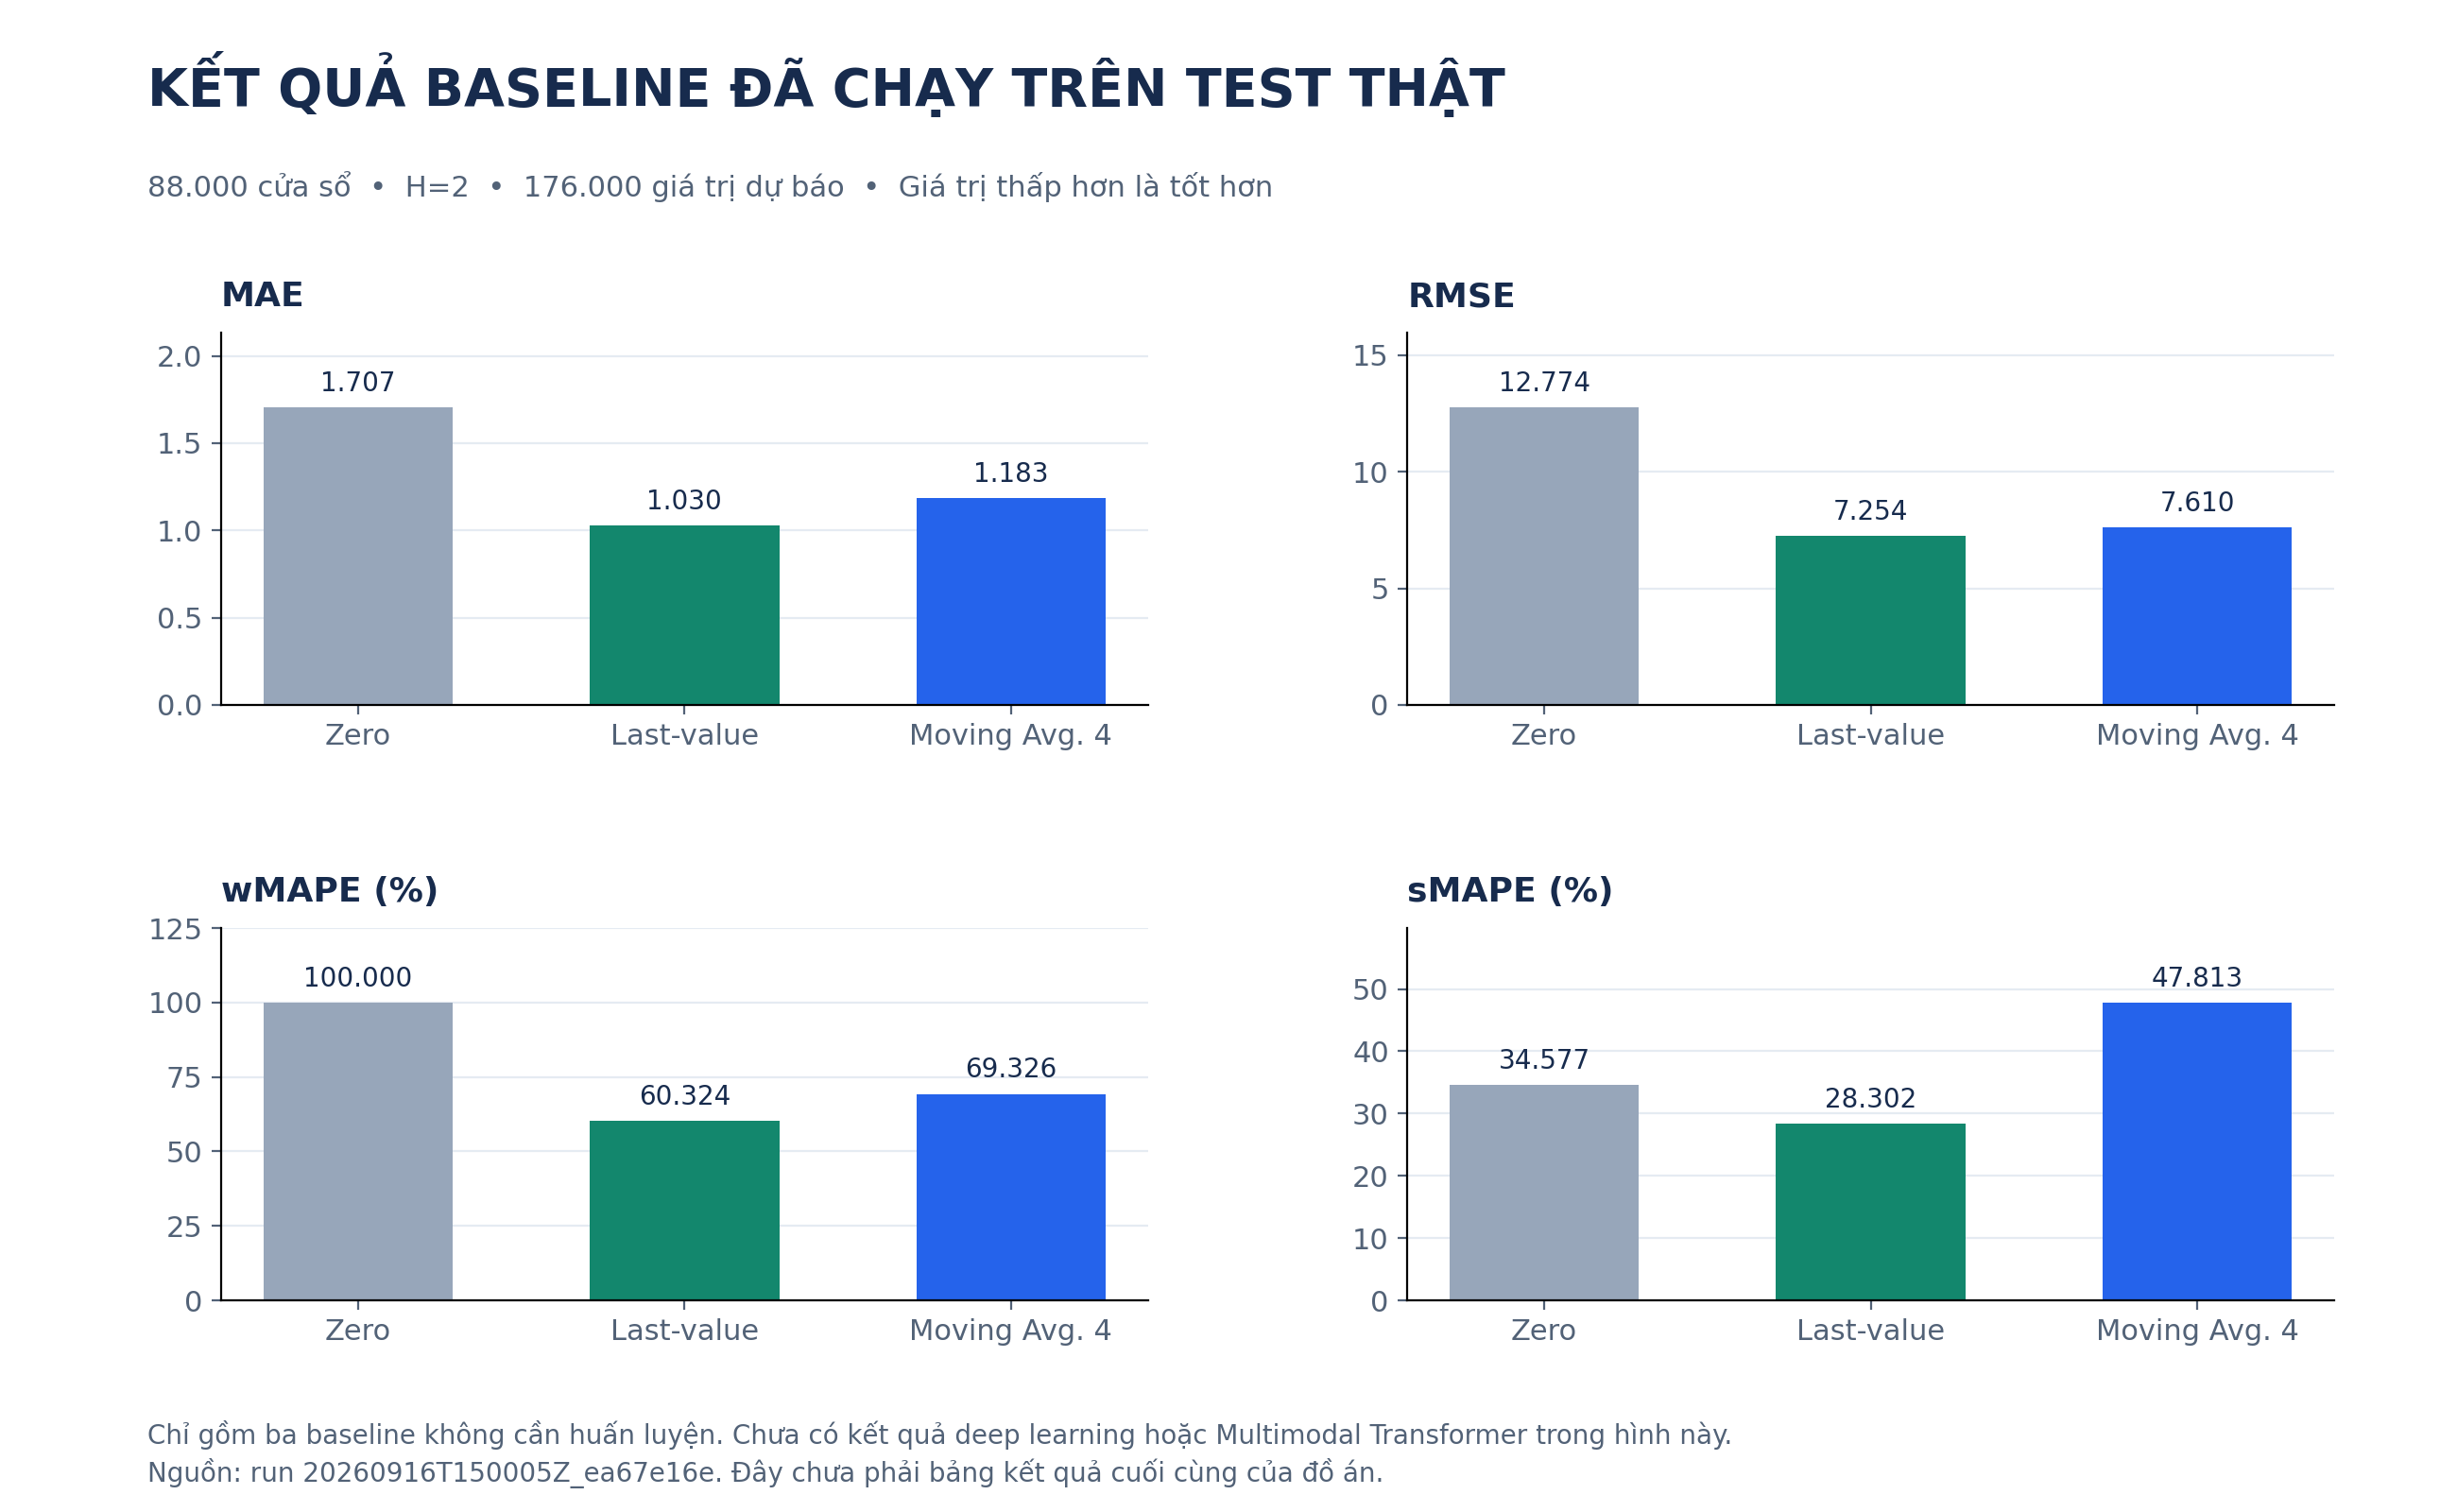
\includegraphics[width=0.92\textwidth]{../../docs/figures/baseline_results_v2.png}
\caption{So sánh các baseline xác định trên cùng tập test.}
\label{fig:naive}
\end{figure}

Hình \ref{fig:naive} lấy từ run \texttt{20260916T150005Z\_ea67e16e} và chỉ minh họa các quy tắc dự báo đơn giản. Bảng \ref{tab:baseline} lấy từ run hoàn tất \texttt{20260920T085601Z\_2c55ebb8} và là nguồn so sánh cho tám mô hình. Hai nguồn được ghi riêng để không gộp kết quả của các lần chạy.

\subsection{Diễn giải so sánh baseline}
Trong run đầy đủ, Temporal Transformer đạt MAE trung bình 0,9381 với độ lệch chuẩn 0,0119; Multimodal MLP đạt 0,9665 với độ lệch chuẩn 0,0043. Khoảng cách MAE giữa hai mô hình vào khoảng 0,0284 đơn vị bán quan sát trên mỗi dự báo. Multimodal MLP có RMSE thấp nhất (6,8016), thấp hơn Temporal Transformer (6,9074), trong khi wMAPE của Transformer thấp hơn (54,97\% so với 56,63\%). Thứ hạng vì thế thay đổi theo metric.

So với Last-value, các mô hình học đều giảm MAE trong run này. Tuy nhiên Moving Average(4) có MAE 1,1832, kém hơn Last-value 1,0296, cho thấy làm trơn lịch sử không tự động cải thiện dự báo. Baseline Zero có RMSE 12,7737, phản ánh các tuần có lượng bán lớn vẫn tạo đóng góp đáng kể vào sai số bình phương. Phân tích này tạo mốc để đánh giá liệu các kiến trúc mới có cải thiện ổn định trên nhiều chỉ số hay chỉ tối ưu một metric.

Các số liệu mean/std từ ba seed giúp phát hiện sự dao động giữa lần train. Multimodal MLP có độ lệch chuẩn MAE thấp trong cấu hình đầy đủ, trong khi một số kịch bản che modality có độ biến thiên lớn hơn. Ba seed là quy mô thăm dò; chưa nên gọi khác biệt nhỏ là có ý nghĩa thống kê nếu chưa có kiểm định phù hợp hoặc thêm lần lặp.

Metric tổng thể gộp hai tuần dự báo thành 176.000 điểm trên toàn bộ tập test. Để làm rõ ảnh hưởng của khoảng cách dự báo, run cũng lưu chỉ số theo horizon cho từng seed. Bảng \ref{tab:horizon-results} tổng hợp MAE và wMAPE của hai mô hình tiêu biểu, tính trung bình $\pm$ độ lệch chuẩn qua ba seed; mỗi horizon có 88.000 điểm dự báo ở mỗi seed.

\begin{table}[!htbp]
\centering
\small
\caption{Kết quả theo bước dự báo trên test; trung bình $\pm$ độ lệch chuẩn qua ba seed.}
\label{tab:horizon-results}
\begin{tabularx}{\textwidth}{p{0.28\textwidth}p{0.19\textwidth}rrX}
\toprule
Mô hình & Tuần dự báo & MAE & wMAPE (\%) & Số điểm mỗi seed \\
\midrule
Transformer chuỗi thời gian & $h=1$ & $0,8481\pm0,0097$ & $47,99\pm0,55$ & 88.000 \\
Transformer chuỗi thời gian & $h=2$ & $1,0281\pm0,0161$ & $62,45\pm0,98$ & 88.000 \\
Multimodal MLP & $h=1$ & $0,8963\pm0,0163$ & $50,71\pm0,92$ & 88.000 \\
Multimodal MLP & $h=2$ & $1,0368\pm0,0079$ & $62,98\pm0,48$ & 88.000 \\
\bottomrule
\end{tabularx}
\end{table}

Ở cả hai mô hình, tuần thứ hai có MAE và wMAPE cao hơn tuần thứ nhất. Đây là xu hướng quan sát trong run này, không phải quy luật được khẳng định cho mọi giai đoạn bán lẻ. Chênh lệch giữa hai kiến trúc cũng thay đổi theo horizon: Transformer thấp hơn Multimodal MLP về MAE ở cả hai bước, trong khi bảng tổng thể cho thấy Multimodal MLP có RMSE thấp hơn. Đọc metric theo từng bước giúp thấy rõ việc gộp các target có thể che đi khác biệt giữa độ gần và xa của dự báo.

Một cách phân tích khác là chia sản phẩm theo tỷ lệ tuần không bán tính riêng trên train: dưới 0,5 và từ 0,5 trở lên. Ngưỡng được xác định trên lịch sử train, tránh dùng nhãn test để tạo nhóm. Do cùng một tập sản phẩm được đánh giá tại 11 origin và hai horizon, hai phân nhóm chứa lần lượt 53.328 và 122.672 điểm dự báo mỗi seed; chúng không phải số lượng mặt hàng.

\begin{table}[!htbp]
\centering
\small
\caption{Kết quả theo độ thưa của lịch sử train; test, trung bình $\pm$ độ lệch chuẩn qua ba seed.}
\label{tab:sparsity-results}
\begin{tabularx}{\textwidth}{p{0.27\textwidth}p{0.18\textwidth}rrX}
\toprule
Mô hình & Tỷ lệ tuần 0 trên train & MAE & wMAPE (\%) & Số điểm mỗi seed \\
\midrule
Transformer chuỗi thời gian & $<0,5$ & $1,9581\pm0,0266$ & $48,74\pm0,66$ & 53.328 \\
Transformer chuỗi thời gian & $\geq0,5$ & $0,4947\pm0,0078$ & $70,45\pm1,11$ & 122.672 \\
Multimodal MLP & $<0,5$ & $1,9778\pm0,0218$ & $49,23\pm0,54$ & 53.328 \\
Multimodal MLP & $\geq0,5$ & $0,5269\pm0,0036$ & $75,04\pm0,51$ & 122.672 \\
\bottomrule
\end{tabularx}
\end{table}

MAE thấp hơn ở nhóm có nhiều tuần 0, trong khi wMAPE thấp hơn ở nhóm hoạt động thường xuyên hơn. Hai chỉ số trả lời những câu hỏi khác nhau: MAE tính sai số trung bình cho từng điểm; wMAPE chia tổng sai số cho tổng lượng bán trong nhóm. Nhóm nhiều số 0 có thể có MAE thấp do phần lớn giá trị gần 0, nhưng mỗi sai số vẫn lớn so với tổng doanh số của nhóm, làm wMAPE cao. Vì vậy không thể diễn giải MAE thấp ở nhóm thưa như bằng chứng chất lượng dự báo cao trên mọi sản phẩm.

Một cách nhìn lý thuyết cho chuỗi bán lẻ thưa là tách hai quá trình: tuần có bán hay không, và bán bao nhiêu nếu có bán. Với $p_{i,t}=P(y_{i,t}>0\mid\mathbf{x}_{i,t})$ và $\mu_{i,t}=E[y_{i,t}\mid y_{i,t}>0,\mathbf{x}_{i,t}]$, kỳ vọng số bán có thể viết thành
\begin{equation}
E[y_{i,t}\mid\mathbf{x}_{i,t}]=p_{i,t}\,\mu_{i,t}.
\end{equation}
Các baseline hiện tại dự báo trực tiếp giá trị đếm, không có hai đầu ra riêng cho xác suất có giao dịch và quy mô khi giao dịch dương. Vì vậy lỗi có thể đến từ dự báo sai trạng thái bán, từ ước lượng sai quy mô, hoặc cả hai. Đây là cách diễn giải cấu trúc dữ liệu và một hướng phân tích tiếp theo; báo cáo chưa có kết quả mô hình hai phần.

Để kiểm tra giả thuyết này ở giai đoạn sau, có thể đánh giá dự báo sự kiện $y>0$ bằng precision/recall hoặc PR-AUC, rồi đánh giá sai số quy mô có điều kiện trên những tuần thực sự có bán. Ngưỡng biến xác suất thành nhãn phải chọn trên validation và giữ cố định khi đo test. Kết quả hai phần cần đặt cạnh MAE/RMSE của mô hình hồi quy trực tiếp, vì hai cách dự báo có mục tiêu tối ưu và cách sử dụng khác nhau.

\subsection{Phân tích thử nghiệm thiếu modality}
Protocol \texttt{same\_checkpoint} lấy cùng một checkpoint Multimodal MLP đã huấn luyện trên đầu vào đầy đủ, sau đó đặt vector modality bị thiếu về 0 tại thời điểm đánh giá. Thiết kế này trả lời câu hỏi độ nhạy của mô hình đã học với việc mất đầu vào; nó không tương đương với huấn luyện mô hình từ đầu trong điều kiện thiếu modality.

Về ký hiệu, có thể mô tả độ sẵn có của ảnh và văn bản bằng hai biến nhị phân $m_i^{img},m_i^{text}\in\{0,1\}$. Cách zero-imputation hiện tại tạo đầu vào $\tilde{\mathbf e}_i=m_i\mathbf e_i$. Khi $m_i=0$, vector bằng không; mô hình không nhận một chỉ dấu tường minh để phân biệt ``modality bị thiếu'' với ``vector có giá trị bằng không''. Một thiết kế mask-token có thể thay thế bằng $\tilde{\mathbf e}_i=m_i\mathbf e_i+(1-m_i)\mathbf q_{miss}$, trong đó $\mathbf q_{miss}$ được học cùng mô hình. Công thức này chỉ mô tả hướng nghiên cứu: run hiện tại dùng zero-imputation, chưa dùng vector $\mathbf q_{miss}$ hoặc modality dropout.

Hai giao thức ablation có ý nghĩa bổ sung nhau. \texttt{same\_checkpoint} cố định tham số $\theta$ và thay đổi đầu vào có sẵn: so sánh $f_\theta(x,m=1)$ với $f_\theta(x,m=0)$. Giao thức \texttt{retrained} thay đổi cả phân bố đầu vào lúc học và tham số ước lượng: $\theta_m=\arg\min_\theta\mathcal{L}_{train}(f_\theta(x,m))$. Giao thức thứ nhất mô phỏng mất đầu vào bất ngờ; giao thức thứ hai đo khả năng thích nghi khi mô hình được huấn luyện cho một tổ hợp modality cố định. Không giao thức nào tự nó chứng minh khả năng bù đắp tổng quát dưới mọi kiểu thiếu dữ liệu.

\begin{table}[!htbp]
\centering
\small
\caption{Độ nhạy khi che modality sau huấn luyện; cùng checkpoint, ba seed.}
\label{tab:missing}
\begin{tabular}{lrrr}
\toprule
Kịch bản đánh giá & MAE trung bình & ĐLC & Thay đổi so với đủ đầu vào \\
\midrule
Đủ đầu vào (26 ảnh thiếu tự nhiên) & 0,9665 & 0,0043 & -- \\
Che ảnh bằng vector 0 & 1,0246 & 0,0549 & +6,0\% \\
Che văn bản bằng vector 0 & 1,0081 & 0,0395 & +4,3\% \\
Che cả ảnh và văn bản & 1,0917 & 0,1128 & +13,0\% \\
Chỉ giữ 6 tuần gần nhất & 0,9891 & 0,0220 & +2,3\% \\
\bottomrule
\end{tabular}
\end{table}

Mức thay đổi được tính theo $100\,(\mathrm{MAE}_{\mathrm{scenario}}-\mathrm{MAE}_{\mathrm{full}})/\mathrm{MAE}_{\mathrm{full}}$ từ trung bình tổng hợp. Khi bỏ ảnh, MAE tăng xấp xỉ 6,0\%; bỏ văn bản tăng 4,3\%; bỏ cả hai tăng 13,0\%. Khi chỉ dùng sáu tuần lịch sử gần nhất, MAE tăng khoảng 2,3\%. Những con số này mô tả một phép gây nhiễu đầu vào sau huấn luyện, không chứng minh mô hình có thể tự bù thông tin. Độ lệch chuẩn của kịch bản thiếu cả hai modality (0,1128) cũng lớn hơn rõ so với baseline đầy đủ (0,0043), gợi ý kết quả nhạy với seed trong đánh giá này.


Run cũng lưu protocol \texttt{retrained}: huấn luyện riêng các phiên bản đầy đủ, thiếu ảnh, thiếu văn bản và thiếu cả hai. Kết quả huấn luyện lại khác câu hỏi với \texttt{same\_checkpoint}; không nên gộp hai giao thức thành một bảng nếu không ghi rõ. Đặc biệt, cần thận trọng khi diễn giải việc bỏ modality làm metric có lúc tốt lên trong giao thức huấn luyện lại: đó có thể là biến động tối ưu và seed, không mặc nhiên là bằng chứng modality có hại.

\begin{table}[!htbp]
\centering
\small
\caption{Ablation Multimodal MLP huấn luyện lại theo modality có sẵn; test, mean $\pm$ độ lệch chuẩn qua ba seed.}
\label{tab:retrained}
\begin{tabular}{lrrr}
\toprule
Đầu vào trong train/validation/test & MAE & RMSE & wMAPE (\%) \\
\midrule
Lịch sử + ảnh + văn bản & $0,9665\pm0,0043$ & $6,8016\pm0,0506$ & $56,63\pm0,25$ \\
Lịch sử + văn bản (thiếu ảnh) & $0,9685\pm0,0081$ & $6,7743\pm0,0381$ & $56,75\pm0,47$ \\
Lịch sử + ảnh (thiếu văn bản) & $0,9574\pm0,0098$ & $6,6881\pm0,0326$ & $56,10\pm0,57$ \\
Chỉ lịch sử (thiếu cả hai) & $0,9732\pm0,0022$ & $6,7550\pm0,0114$ & $57,02\pm0,13$ \\
\bottomrule
\end{tabular}
\end{table}

Trong giao thức huấn luyện lại, các cấu hình thiếu ảnh hoặc thiếu văn bản không suy giảm MAE so với đầy đủ; cấu hình chỉ dùng lịch sử có MAE cao nhất trong bốn cấu hình nhưng chênh lệch nhỏ. Đây không phải mâu thuẫn với Bảng \ref{tab:missing}: bảng đó đánh giá cùng checkpoint, còn Bảng \ref{tab:retrained} cho phép mỗi cấu hình học trọng số riêng. Khả năng thích nghi qua huấn luyện và độ nhạy khi mất đầu vào sau khi huấn luyện là hai khía cạnh khác nhau.

\section{Thảo luận và giới hạn}
\subsection{Ý nghĩa kết quả hiện tại}
Kết quả cho thấy các mô hình học giảm MAE so với hai baseline gần nhất trên tập kiểm tra, trong khi mô hình dự báo 0 yếu hơn đáng kể theo MAE và RMSE. Transformer chuỗi thời gian đạt MAE tốt nhất trong nhóm học; Multimodal MLP đạt RMSE tốt nhất. Chênh lệch này nhấn mạnh rằng thứ hạng phụ thuộc metric, do đó báo cáo cuối cần trình bày đồng thời nhiều chỉ số và phân tích theo horizon/nhóm sản phẩm.

Tỷ lệ 0 cao khiến các chỉ số gộp chịu ảnh hưởng lớn từ tuần không bán. wMAPE vẫn ở khoảng 55--57\% cho các mô hình học, và sMAPE trên các mô hình học gần 170--179\%. MAE nhỏ hơn một đơn vị không nên diễn giải như dự báo chính xác cho mọi sản phẩm: sai số tập trung ở phân phối có đuôi dài có thể bị che khuất bởi số lượng lớn giá trị 0. Vì vậy, phân tích tiếp theo cần tách tuần bán/không bán, nhóm sản phẩm, tuần dự báo thứ nhất/thứ hai và mức hoạt động lịch sử.

Một cách đọc bổ sung là xem kết quả theo từng bước dự báo. Khi $H=2$, mô hình tạo hai giá trị tương lai cho mỗi origin; gộp hai horizon thành một metric có thể che giấu việc dự báo tuần kế tiếp tốt hơn tuần thứ hai. Tương tự, gộp 14 nhóm sản phẩm làm nhóm có hàng nghìn mã chi phối kết quả. Do vậy báo cáo cuối nên có metric theo horizon và nhóm, kèm số dự báo trong từng ô. Nếu nhóm có tổng lượng thật bằng 0, cần để trống wMAPE thay vì thay bằng 0 để tránh tạo ấn tượng mô hình không có lỗi.

Kết quả hiện tại cũng chưa tách tác động của embedding khỏi khác biệt kiến trúc hoặc số tham số. So sánh công bằng nên giữ cố định split, target transform và seed; sau đó so sales-only MLP với Multimodal MLP có cùng khung dự báo, kiểm tra mask availability, và báo cáo ablation train lại. Các thí nghiệm hiện có là bước chuẩn bị hữu ích nhưng chưa đủ để kết luận ảnh hay văn bản cải thiện chất lượng dự báo trong mọi trường hợp.

\subsection{Các giới hạn}
\begin{itemize}
  \item Nhãn là số giao dịch ghi nhận, không phải nhu cầu chưa bị giới hạn bởi tồn kho; dữ liệu hiện tại không cho biết mặt hàng có hết hàng hay không.
  \item Mẫu chỉ gồm các sản phẩm có đủ hoạt động và giao dịch trong train; kết quả chưa đại diện cho cold-start hoặc sản phẩm hiếm.
  \item Có 26 ảnh thiếu tự nhiên và 38 mô tả chi tiết rỗng trong mẫu; các trường hợp này cần được giữ trong báo cáo độ phủ.
  \item Baseline đa phương thức là MLP ghép đặc trưng, chưa có token-level fusion, cross-attention, learnable mask token hay contrastive alignment.
  \item Ba seed cung cấp ước lượng độ ổn định ban đầu, nhưng chưa phải kiểm định thống kê và chưa bảo đảm kết quả khái quát ngoài phép chia hiện tại.
\end{itemize}

\subsection{Hướng mở rộng bám theo giới hạn}
Các giới hạn nêu trên dẫn đến một thứ tự thực nghiệm cụ thể. Trước hết cần cố định lại nguồn embedding, ghi model revision, cấu hình tiền xử lý và hash của danh sách sản phẩm; sau đó hoàn thành bảng metric theo horizon và nhóm. Khi đường cơ sở ổn định, mới xây kiến trúc fusion để phân biệt lợi ích của việc dùng modality với lợi ích riêng của kiến trúc. Cuối cùng, missing-modality training được đánh giá trên cùng danh sách mặt nạ và cùng seed với zero-imputation.

\begin{table}[!htbp]
\centering
\small
\caption{Lộ trình thí nghiệm tiếp theo và bằng chứng cần lưu.}
\label{tab:roadmap}
\begin{tabularx}{\textwidth}{p{0.20\textwidth}p{0.34\textwidth}X}
\toprule
Thứ tự & Công việc & Bằng chứng để báo cáo \\
\midrule
1 & Hoàn thiện provenance và phân tích theo horizon/nhóm & Model revision, hash đầu vào, CSV metric có số mẫu cho từng horizon và nhóm. \\
2 & So sánh sales-only và fusion trên cùng split & Cấu hình, checkpoint, seed và bảng MAE/RMSE/wMAPE/sMAPE. \\
3 & Thêm availability mask hoặc token thiếu & Kiểm tra phân biệt thiếu tự nhiên với vector số 0 hợp lệ. \\
4 & Huấn luyện modality dropout & Kịch bản che cố định, đối chứng zero-imputation và kết quả trung bình/độ lệch chuẩn. \\
5 & Phân tích cơ chế fusion & Attention/ablation chỉ trình bày nếu được trích xuất từ mô hình thực nghiệm. \\
\bottomrule
\end{tabularx}
\end{table}

Sơ đồ dưới đây khái quát một phương án cho Stage 4--5: mã hóa riêng từng nguồn, chiếu chúng về số chiều chung, dùng cờ sẵn có để thay nguồn vắng mặt bằng token học được, rồi hợp nhất bằng Transformer và dự báo hai tuần. Sơ đồ là thiết kế để triển khai và kiểm chứng, không phải mô hình đã được huấn luyện trong run Stage 3.

\begin{figure}[H]
\centering
\begin{tikzpicture}[
  box/.style={draw=hcmutblue,rounded corners=2pt,fill=blue!4,align=center,
              text width=2.15cm,minimum height=0.85cm,font=\footnotesize,inner sep=4pt},
  fusion/.style={draw=hcmutblue,rounded corners=2pt,fill=blue!10,align=center,
              text width=2.4cm,minimum height=1.05cm,font=\small,inner sep=4pt},
  arrow/.style={-{Stealth[length=2mm]},thick,hcmutblue},
  maskarrow/.style={-{Stealth[length=2mm]},thick,dashed,orange!85!black}]
  \node[box] (hist) at (0,2.1) {12 tuần bán\\theo thời gian};
  \node[box] (image) at (0,0.7) {Embedding ảnh\\768 chiều};
  \node[box] (text) at (0,-0.7) {Embedding văn bản\\384 chiều};
  \node[box] (ph) at (3.0,2.1) {Chiếu chuỗi\\về không gian chung};
  \node[box] (pi) at (3.0,0.7) {Chiếu ảnh\\về không gian chung};
  \node[box] (pt) at (3.0,-0.7) {Chiếu văn bản\\về không gian chung};
  \node[box,fill=orange!8,draw=orange!85!black] (mask) at (6.1,-1.9) {Token thiếu\\được học};
  \node[fusion] (encoder) at (7.0,0.8) {Hợp nhất token\\bằng Transformer};
  \node[fusion] (head) at (10.3,0.8) {Đầu dự báo\\hai horizon};
  \node[box] (out) at (13.1,0.8) {$\hat y_{t+1},\hat y_{t+2}$};
  \draw[arrow] (hist) -- (ph);
  \draw[arrow] (image) -- (pi);
  \draw[arrow] (text) -- (pt);
  \draw[arrow] (ph.east) -- ++(0.45,0) |- (encoder.west);
  \draw[arrow] (pi.east) -- (encoder.west);
  \draw[arrow] (pt.east) -- ++(0.45,0) |- (encoder.west);
  \draw[maskarrow] (mask.north) -- ++(0,0.45) -| (encoder.south);
  \draw[arrow] (encoder) -- (head);
  \draw[arrow] (head) -- (out);
\end{tikzpicture}
\caption{Sơ đồ khái niệm cho mô hình đa phương thức chịu thiếu dữ liệu; các projection, token thiếu và Transformer fusion chưa được triển khai trong kết quả hiện tại.}
\label{fig:proposed-architecture}
\end{figure}

Thiết kế cần được kiểm tra theo từng thành phần thay vì thay đồng thời nhiều lựa chọn. Trước hết xác nhận mô hình full-modality có cải thiện sales-only khi giữ nguyên kích thước train, split và seed. Tiếp đó bật masking nhưng chưa dùng loss căn chỉnh để đo riêng giá trị của token thiếu. Cuối cùng mới thêm alignment nếu có giả thuyết về tương đồng ảnh-văn bản và một đối chứng ablation loại bỏ loss này. Thứ tự này giảm nguy cơ gán mức cải thiện cho sai thành phần.

Lộ trình này ưu tiên các đối chứng có thể kiểm tra và tái lập trước các kỹ thuật phức tạp. Prompt tuning hoặc contrastive alignment chỉ nên thêm nếu fusion cơ sở và modality dropout đã được đánh giá rõ; nếu đưa vào, cần thiết kế loss và thí nghiệm riêng để biết cải thiện đến từ đâu.

\clearpage
\clearpage
\section*{Tóm tắt tiến độ}
Đã hoàn thành dữ liệu tuần H\&M v2 cho 8.000 sản phẩm, tạo embedding văn bản cho đủ 8.000 sản phẩm và embedding ảnh đọc được cho 7.974 sản phẩm. Stage 3 đã chạy ba baseline xác định, bốn mô hình đơn phương thức/chuỗi và Multimodal MLP qua ba seed; cùng checkpoint và huấn luyện lại đều có ablation thiếu modality. Kết quả là mốc giữa kỳ: mô hình đa phương thức hiện tại là MLP ghép đặc trưng, chưa phải Transformer đa phương thức; cơ chế học để chịu thiếu modality còn nằm trong kế hoạch tiếp theo.
\vspace{0.5cm}

\section*{Báo cáo tiến độ thực hiện}
\addcontentsline{toc}{section}{Báo cáo tiến độ thực hiện}
\begin{table}[!htbp]
\centering
\caption{Tình trạng các giai đoạn và công việc tiếp theo.}
\label{tab:progress}
\begin{tabularx}{\textwidth}{p{0.20\textwidth}p{0.17\textwidth}X}
\toprule
Giai đoạn & Tình trạng & Kết quả đã đạt / công việc tiếp theo \\
\midrule
1. Dữ liệu & Hoàn thành & EDA; chọn mẫu chỉ từ train; gom tuần, zero-fill và chia 80/12/12 tuần. \\
2. Embedding & Đã chạy & Tạo vector ảnh/văn bản và audit độ phủ; cần bổ sung revision CLIP đã resolve để provenance đầy đủ. \\
3. Baseline & Đã chạy & 8 mô hình; các mô hình học chạy ba seed; có ablation giữ checkpoint và huấn luyện lại. \\
4. Transformer đa phương thức & Tiếp theo & Chiếu các nguồn về không gian chung; so sánh ghép token với cơ chế chú ý chéo. \\
5. Học khi thiếu dữ liệu & Đang thiết kế & Thử token thiếu được học và dropout modality; đối chiếu với thay vector bằng 0. \\
6. Đánh giá và báo cáo & Đang thực hiện & Phân tích theo nhóm, horizon và độ thưa; hoàn thiện bảng ablation, hình và phần giới hạn. \\
\bottomrule
\end{tabularx}
\end{table}

\subsection*{Nguyên tắc cho các thí nghiệm tiếp theo}
Các phương pháp cần dùng cùng split, horizon và tập sản phẩm; chạy trên cùng danh sách seed; báo cáo đồng thời MAE, RMSE, wMAPE, sMAPE và độ phủ modality. Với tình huống cắt lịch sử, cần có baseline chuỗi thời gian bị cắt đúng cùng số tuần để đối chiếu công bằng. Các thiết kế Transformer đa phương thức và modality dropout là kế hoạch, chưa phải kết quả đã chạy.

Mỗi lần chạy cần lưu cấu hình đầy đủ, mã nguồn hoặc commit, thời gian thực thi, phiên bản thư viện, kết quả theo seed và dự báo ở mức mẫu để có thể kiểm tra lại metric tổng hợp. Với embedding tải từ Kaggle, cần ghi nguồn dataset, tên encoder và revision thực tế; không chỉ ghi tên thư viện. Khi trình bày kết quả, nên nêu rõ run ID và protocol ngay trong caption hoặc phần mô tả bảng.

\clearpage
\section{Kết luận tiến độ}
Đến thời điểm lập báo cáo, pipeline đã tạo được dữ liệu tuần v2 cho 8.000 sản phẩm, hoàn thành trích xuất và kiểm định embedding ảnh/văn bản với độ phủ ảnh được ghi nhận rõ, đồng thời chạy xong các baseline và ablation Stage 3 trên dữ liệu thật. Kết quả cung cấp mốc định lượng ban đầu và cho thấy sai số thay đổi khi đầu vào đa phương thức bị loại bỏ.

Đóng góp cốt lõi vẫn ở phía trước: xây dựng Multimodal Transformer và cơ chế học trong điều kiện thiếu modality, sau đó đối chiếu bằng ablation có kiểm soát. Báo cáo vì vậy trình bày các kết quả Stage 3 như bằng chứng tiến độ, không gọi baseline hiện tại là mô hình đề xuất hoàn chỉnh.

\section{Nguồn dữ liệu }
\begin{table}[!htbp]
\centering
\small
\caption{Nguồn và vị trí kiểm tra số liệu trong project.}
\begin{tabularx}{\textwidth}{p{0.23\textwidth}X}
\toprule
Nguồn & Tài liệu \\
\midrule
Bộ dữ liệu & \href{https://www.kaggle.com/competitions/h-and-m-personalized-fashion-recommendations}{H\&M Personalized Fashion Recommendations trên Kaggle} \\
Notebook chạy & \href{https://www.kaggle.com/code/alexnguyen147/datn-notebook}{Notebook DATN của Nguyễn Vũ Quang Minh} \\
Tóm tắt Stage 1 & \texttt{processed\_data/v2/stage1\_summary.json}: quy tắc chọn mẫu, tuần, split và tỷ lệ zero. \\
Run Stage 3 & \texttt{results/v2/20260920T085601Z\_2c55ebb8/}: cấu hình, metric tổng hợp/theo nhóm và so sánh robustness. \\
Mã xây dựng dữ liệu & \texttt{src/data/build\_weekly\_sales.py}, \texttt{src/data/select\_articles.py}, \texttt{src/data/dataset.py}. \\
Mã train và metric & \texttt{src/pipeline/train\_baselines.py}, \texttt{src/utils/trainer.py}, \texttt{src/utils/metrics.py}. \\
Đồ thị báo cáo & \texttt{docs/figures/figure\_sources.json} ghi file nguồn của các hình EDA và baseline. \\
Kho mã & \href{https://github.com/minhquangAlex/DATN-Multimodal-Transformer}{Mã nguồn và tài liệu project trên GitHub} \\
Slide tiến độ & \href{https://www.canva.com/design/DAHXzrrA_dY/iwDhfMl-jzznss1wrkEeXw/edit}{Bài thuyết trình tiến độ trên Canva} \\
\bottomrule
\end{tabularx}
\end{table}

\end{document}
